\documentclass[a4paper,11pt]{article}
% !TeX program = pdflatex
\pdfoutput=1
\pdfminorversion=7
\usepackage[utf8]{inputenc}
\usepackage{CJKutf8}
\AtBeginDocument{\begin{CJK*}{UTF8}{gbsn}}
\AtEndDocument{\clearpage\end{CJK*}}
\usepackage{jheppub}

\usepackage{amsmath,amssymb,latexsym}
\usepackage{braket}
\usepackage{bm}
\usepackage{booktabs}
\usepackage{cancel}
\usepackage[svgnames]{xcolor}
\usepackage{hepunits}
\usepackage{mathtools}
\usepackage{graphicx}
\usepackage[most]{tcolorbox}
\usepackage{caption}
\usepackage{tikz}
\usetikzlibrary{calc}
\graphicspath{{./}{000_note/}}
\def\ie{\begin{equation}\begin{aligned}}
\def\fe{\end{aligned}\end{equation}}
\newtcolorbox{proofbox}{
  enhanced, breakable, colback=gray!8, colframe=black,
  boxrule=0.8pt, arc=0pt, outer arc=0pt,
  left=8pt, right=8pt, top=8pt, bottom=8pt,
  before skip=10pt, after skip=10pt
}
\hypersetup{colorlinks=true,linkcolor=blue,citecolor=blue,urlcolor=blue}

\title{Massless Loop dS}
\author[a]{Su Yingze}
\affiliation[a]{Institute not specified}
\emailAdd{yingze.su@outlook.com}
\abstract{研究 de Sitter 时空中 massless 标量场关联函数的 IBP 约化与微分方程，涵盖圈图阶，同时处理原始时间编序（tq 表示）和 kinematic-flow 能量（xq 表示）两种形式。}

\begin{document}
\maketitle
\tableofcontents
\newpage

% ============================================================
\section{背景与 Feynman 规则}
% ============================================================

\subsection{FRW 时空与 conformal scalar}

考虑 $(d+1)$ 维幂律 FRW 时空，其空间平直度规为
\begin{equation}
    ds^2=-dt^2+a^2(t)d\boldsymbol{x}^2,
\end{equation}
其中 $\boldsymbol{x}\in\mathbb{R}^d$，标度因子取
\begin{equation}
    a(t)=\Bigl(\frac{t}{t_0}\Bigr)^p.
\end{equation}
通过 $d\tau=dt/a(t)$ 转换到共形时间 $\tau$，
\begin{equation}
    a(\tau)=\Bigl(\frac{\tau}{\tau_0}\Bigr)^{\tilde{p}},\qquad \tilde{p}\equiv\frac{p}{1-p},
\end{equation}
度规化为
\begin{equation}
    ds^2=a^2(\tau)(-d\tau^2+d\boldsymbol{x}^2).
\end{equation}

对与 Ricci 标量 $R$ 非最小耦合的 massless scalar（即 conformal scalar），作用量为
\begin{equation}
    S[\phi]=\int d^{d+1}x\sqrt{-g}\Bigl[\frac12(\partial_\mu\phi)^2+\frac12\xi R\phi^2+\sum_{n\ge3}\frac{g_n}{n!}\phi^n\Bigr],
\end{equation}
其中 $\xi\equiv(d-1)/4d$。经场重定义 $\phi=a^{(1-d)/2}(\tau)\varphi$，作用量约化为
\begin{equation}
    S[\varphi]=-\int d\tau d^d\boldsymbol{x}\Bigl[\frac12(\partial_\mu\varphi)^2+\sum_{n\ge3}\frac{g_n(-\tau)^{a-1}}{n!}\varphi^n\Bigr].
\end{equation}
这里 $g_n$ 是整体耦合常数，在积分族分析中不参与 IBP/DE；$a-1$ 是该固定相互作用顶点的有效时间幂次，由背景标度因子和场重定义共同决定。后文只保留影响函数族的幂次 $a_i$。

\subsection{Schwinger-Keldysh 形式与 conformal scalar Feynman 规则}

利用 Schwinger-Keldysh (SK) 闭时路径形式，$n$ 点关联函数为
\begin{gather}
    \langle\varphi(\boldsymbol{k}_1)\cdots\varphi(\boldsymbol{k}_n)\rangle'(2\pi)^d\delta^{(d)}(\boldsymbol{k}_1+\cdots+\boldsymbol{k}_n)\notag\\
    =\int\mathcal{D}\varphi_+\mathcal{D}\varphi_-\;\varphi(\tau_f,\boldsymbol{k}_1)\cdots\varphi(\tau_f,\boldsymbol{k}_n)\,e^{iS[\varphi_+]-iS[\varphi_-]}\prod_{\boldsymbol{k}}\delta[\varphi_+(\tau_f,\boldsymbol{k})-\varphi_-(\tau_f,\boldsymbol{k})].
\end{gather}

顶点时间 $\tau_i$ 从 $-\infty$（渐近过去）积到 $0$（未来），两条 SK 分支的顶点因子为
\begin{equation}
    +\text{ 顶点}: -ig_n(-\tau_i)^{a_i-1},\qquad
    -\text{ 顶点}: +ig_n(-\tau_i)^{a_i-1}.
\end{equation}
bulk propagator 有四种符号选择：
\begin{align}
D_{\pm\pm}(k;\tau_1,\tau_2)
&=\frac{1}{2k}\Bigl[e^{\mp ik(\tau_1-\tau_2)}\theta(\tau_1-\tau_2)+e^{\pm ik(\tau_1-\tau_2)}\theta(\tau_2-\tau_1)\Bigr],\\
D_{\pm\mp}(k;\tau_1,\tau_2)
&=\frac{1}{2k}e^{\pm ik(\tau_1-\tau_2)}.
\end{align}
Conformal scalar 的 bulk-to-boundary propagator 为
\begin{equation}
    D_{\pm}(k;\tau)=\frac{1}{2k}e^{\pm ik\tau}.
\end{equation}
其中 $k=|\boldsymbol{k}|$ 为空间动量大小。

\subsection{Wavefunction conformal scalar Feynman 规则}

kinematic-flow 文献处理的基准对象是 conformal scalar 的 wavefunction coefficient，而不是上面的 SK correlator。设晚时边界在 $\tau_f\to0$，wavefunction 写为
\begin{equation}
    \Psi[\phi]=
    \exp\left[-\sum_{m\ge2}\frac{1}{m!}\int\prod_{r=1}^{m}\frac{d^d\boldsymbol{k}_r}{(2\pi)^d}\,
    \phi(\boldsymbol{k}_r)\,
    \psi_m(\boldsymbol{k}_1,\dots,\boldsymbol{k}_m)
    (2\pi)^d\delta^{(d)}\!\left(\sum_{r=1}^{m}\boldsymbol{k}_r\right)\right].
\end{equation}
这里 $\psi_m$ 是 wavefunction coefficient；晚时 correlator 则由 $|\Psi[\phi]|^2$ 的统计平均得到，因此二者不是同一个函数族。对 conformal scalar，取去掉外部归一化后的 wavefunction 规则为 \cite{Fan:2024frw,Hang:2024frw,Baumann:2024loop}
\begin{align}
    K(E;\tau)&=e^{iE\tau},\\
    G(E;\tau,\tau')&=\frac{1}{2E}\Bigl[
    e^{-iE(\tau-\tau')}\theta(\tau-\tau')
    +e^{iE(\tau-\tau')}\theta(\tau'-\tau)
    -e^{iE(\tau+\tau')}
    \Bigr].
    \label{wfpropagators}
\end{align}
其中 $K$ 是 bulk-to-boundary 传播子，$G$ 是 wavefunction bulk-to-bulk 传播子。与 SK propagator 相比，$G$ 多出边界条件项 $-e^{iE(\tau+\tau')}$，使任一端点趋近晚时边界时传播子满足 wavefunction 的 Dirichlet 条件。每个顶点给出 $i\lambda_v(-\tau_v)^{a_v-1}$ 并对 $\tau_v\in(-\infty,0)$ 积分；下文做 IBP/DE 时省略整体耦合常数。

对任意 $N$-site、$L$-loop 图 $\Gamma$，令 $V_\Gamma$ 和 $E_\Gamma$ 分别表示顶点集合和内线集合，$k_v$ 表示流入顶点 $v$ 并到达晚时边界的外部能量和，内线能量统一写成对应动量的模长 $|\boldsymbol{p}_e|$。固定 loop integrand 后，其 flat-space wavefunction integrand 可写为
\begin{equation}
    \widetilde{\psi}^{\rm flat}_{(N,L)}[k_v,|\boldsymbol{p}_e|]
    =
    i^N\int_{-\infty}^{0}\prod_{v\in V_\Gamma}d\tau_v\,
    \prod_{v\in V_\Gamma}K(k_v;\tau_v)
    \prod_{e\in E_\Gamma}G(|\boldsymbol{p}_e|;\tau_{v_e},\tau_{v'_e}).
    \label{flatwfgen}
\end{equation}
该式是后文和 kinematic flow 对比的基准公式；本项目当前的 massless correlator 函数族只借用它的能量超平面结构，不能把它当作 SK correlator 的 Feynman 规则。

\subsection{Massless scalar Feynman 规则}

对于作为圈图内线的 massless scalar $\sigma$，考虑其与 conformal scalar 的 contact interaction：
\begin{equation}
    \mathcal{L}\supset -\frac{\lambda_{n,2}}{n!2!}a^{4-n}(\tau)\varphi^n\sigma^2,
\end{equation}
其中 $a(\tau)=-(H\tau)^{-1}$（下文取 $H=1$）。对 $(3+1)$ 维，$\sqrt{-g}=a^4(\tau)$，conformal scalar 场重定义为 $\phi_c=a^{-1}(\tau)\varphi$。为 IBP 分析方便，采用去掉耦合常数和对称因子的通用相互作用形式：
\begin{equation}
    S_{\text{int}}=\int d\tau d\boldsymbol{x}\,(-\tau)^{a_i-1}\varphi^n\sigma^2.
\end{equation}
指数 $a_i-1$ 表示该顶点处的有效时间幂次；在具体图中，每个顶点的幂次由相互作用和连到该顶点的传播子多项式共同决定。

Massless scalar 的 mode function（$H=1$）为
\begin{equation}
    u_k(\tau)=\frac{1}{\sqrt{2k^3}}(1+ik\tau)e^{-ik\tau},\qquad
    u_k^*(\tau)=\frac{1}{\sqrt{2k^3}}(1-ik\tau)e^{+ik\tau}.
\end{equation}
由 SK 构造，Wightman 函数为
\begin{equation}
    G_>(k;\tau_1,\tau_2)=u_k(\tau_1)u_k^*(\tau_2),\qquad
    G_<(k;\tau_1,\tau_2)=u_k^*(\tau_1)u_k(\tau_2),
\end{equation}
树图 bulk propagator 为
\begin{align}
D_{\pm\pm}(k;\tau_1,\tau_2)&=\frac{1}{2k^3}\Bigl[(1\pm ik\tau_1)(1\mp ik\tau_2)e^{\mp ik(\tau_1-\tau_2)}\theta(\tau_1-\tau_2)\notag\\
&\qquad\qquad+(1\mp ik\tau_1)(1\pm ik\tau_2)e^{\pm ik(\tau_1-\tau_2)}\theta(\tau_2-\tau_1)\Bigr],\\
D_{\pm\mp}(k;\tau_1,\tau_2)&=\frac{1}{2k^3}(1\mp ik\tau_1)(1\pm ik\tau_2)e^{\pm ik(\tau_1-\tau_2)}.
\end{align}
Massless 外腿的 bulk-to-boundary propagator（圈图计算中不使用，但列出供参考）为
\begin{equation}
    B_{\pm}(k;\tau)=\frac{1\mp ik\tau}{2k^3}e^{\pm ik\tau}.
\end{equation}

以上 conformal scalar 和 massless scalar 的 Feynman 规则属于统一的积分函数族——两者仅在传播子分母的 $k$ 幂次（$1/2k$ vs $1/2k^3$）和时间多项式因子 $(1\pm ik\tau)$ 的有无上不同。后续各章的 IBP 和 DE 讨论针对的是该函数族的通用结构，不再区分两种标量场。wavefunction coefficient 与 correlator 的 Feynman 规则在 bulk-to-boundary 传播子的边界条件上可能存在差异，相关结论需在使用具体 kinematic-flow 规则时逐项确认。

\subsection{维度正规化与运动学约定}

我们在 $d$ 维空间中工作，全程使用维度正规化。偏离物理维度的参数为
\begin{equation}
    \epsilon\equiv d-3\qquad(\text{对 }d=3\text{ 外维度}),
\end{equation}
或更一般地通过标度因子指数体现。$\epsilon=0,-1,-2,-3$ 分别对应于 de Sitter、Minkowski、辐射主导和物质主导宇宙。标度因子取幂律形式
\begin{equation}
    a(\tau)=\tau^{-(1+\epsilon)},
\end{equation}
后文的 IBP/DE 只依赖函数族中的时间幂次 $a_i$ 和分母幂次，不需要保留整体耦合常数。

对下文的 2-site 1-loop bubble，单圈两条内线的模长统一记为
\begin{equation}
    q_1=|\boldsymbol{q}|,\qquad q_2=|\boldsymbol{q}+\boldsymbol{k}_3|.
    \label{qidef}
\end{equation}
也就是说，$\boldsymbol{q}$ 仍是圈动量矢量，$q_1,q_2$ 只表示两条内传播子的能量模长。

\subsection{Family tree 分解}

Family tree 分解利用恒等式
\begin{equation}
    \theta(\tau_i-\tau_j)+\theta(\tau_j-\tau_i)=1
\end{equation}
消去冗余的 Heaviside 函数。在 conformal scalar bubble 的 $(++)$ 构型中，四个传播子因子（每条内线两个）的乘积约化为
\begin{equation}
    \bigl[e^{-i(q_1+q_2)(\tau_1-\tau_2)}\theta(\tau_1-\tau_2)+e^{i(q_1+q_2)(\tau_1-\tau_2)}\theta(\tau_2-\tau_1)\bigr],
\end{equation}
仅通过 $q_1+q_2$ 依赖于内线动量。$(++)$ 构型的时间被积函数因此化为
\begin{multline}
    \Bigl[
    e^{i(k_1+q_1+q_2)\tau_1}
    e^{i(k_2-q_1-q_2)\tau_2}
    -e^{i(k_1-q_1-q_2)\tau_1}
    e^{i(k_2+q_1+q_2)\tau_2}
    \Bigr]\theta(\tau_2-\tau_1)\\
    +e^{i(k_1-q_1-q_2)\tau_1}
    e^{i(k_2+q_1+q_2)\tau_2}.
\end{multline}
详细推导（含嵌套时间积分的 Mellin-Barnes 处理）见附录 A。


\newpage
% ============================================================
\section{从 tq 表示到 xq 表示}
% ============================================================

我们研究的是 2-site 1-loop bubble 图：两个顶点（分别有 $n_1$ 和 $n_2$ 条外线，$n_1+n_2=n$），由两条内线连接形成单圈。圈动量记为 $\boldsymbol{q}$，两条内线的动量分别为 $\boldsymbol{q}$ 和 $\boldsymbol{q}+\boldsymbol{k}_3$。所有外动量取全部流入约定 $\boldsymbol{k}_1+\cdots+\boldsymbol{k}_n=0$。

\begin{center}
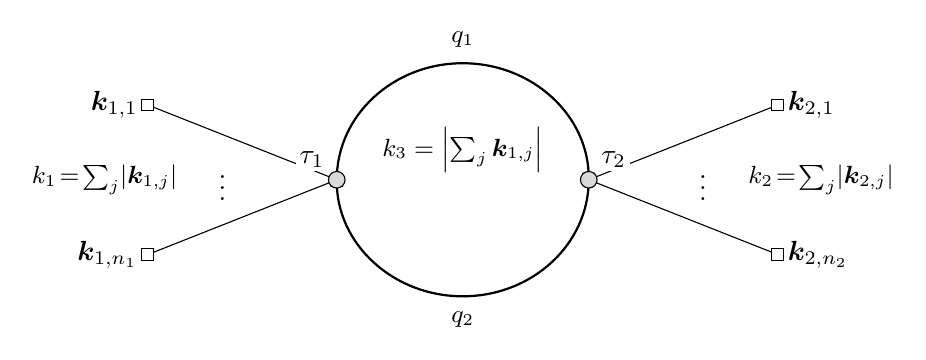
\begin{tikzpicture}[scale=1.0, every node/.style={inner sep=1.5pt}]
  \coordinate (vL) at (0,0);
  \coordinate (vR) at (3.2,0);
  \coordinate (lU) at (-2.4,0.95);
  \coordinate (lD) at (-2.4,-0.95);
  \coordinate (rU) at (5.6,0.95);
  \coordinate (rD) at (5.6,-0.95);
  \draw (vL) -- (lU) node[left=2pt] {$\boldsymbol{k}_{1,1}$};
  \draw (vL) -- (lD) node[left=2pt] {$\boldsymbol{k}_{1,n_1}$};
  \draw (vR) -- (rU) node[right=2pt] {$\boldsymbol{k}_{2,1}$};
  \draw (vR) -- (rD) node[right=2pt] {$\boldsymbol{k}_{2,n_2}$};
  \node[fill=white,inner sep=1pt] at (-1.45,0) {$\vdots$};
  \node[fill=white,inner sep=1pt] at (4.65,0) {$\vdots$};
  \draw[->,thick] (vL) arc[start angle=180,end angle=0,x radius=1.6,y radius=1.48];
  \draw[->,thick] (vR) arc[start angle=0,end angle=-180,x radius=1.6,y radius=1.48];
  \node[fill=white] at (1.6,1.78) {\small $q_1$};
  \node[fill=white] at (1.6,-1.78) {\small $q_2$};
  \node[fill=white] at (1.6,0.38) {\small $k_3=\left|\sum_j\boldsymbol{k}_{1,j}\right|$};
  \node[fill=white] at (-2.95,0) {\small $k_1\!=\!\sum_j\!|\boldsymbol{k}_{1,j}|$};
  \node[fill=white] at (6.15,0) {\small $k_2\!=\!\sum_j\!|\boldsymbol{k}_{2,j}|$};
  \filldraw[fill=gray!30,draw=black] (vL) circle (3pt);
  \filldraw[fill=gray!30,draw=black] (vR) circle (3pt);
  \node[fill=white,anchor=south east] at (-0.10,0.10) {$\tau_1$};
  \node[fill=white,anchor=south west] at (3.30,0.10) {$\tau_2$};
  \filldraw[fill=white,draw=black] ($(lU)+(-0.075,0.075)$) rectangle ++(0.15,-0.15);
  \filldraw[fill=white,draw=black] ($(lD)+(-0.075,0.075)$) rectangle ++(0.15,-0.15);
  \filldraw[fill=white,draw=black] ($(rU)+(-0.075,0.075)$) rectangle ++(0.15,-0.15);
  \filldraw[fill=white,draw=black] ($(rD)+(-0.075,0.075)$) rectangle ++(0.15,-0.15);
\end{tikzpicture}
\end{center}

\textbf{运动学参量。} 被积函数中永远绑定出现的外动量之和记为：
\begin{equation}
    k_1=\sum_{j=1}^{n_1} k_{1,j},\qquad k_2=\sum_{j=1}^{n_2} k_{2,j},\qquad k_{1,j}\equiv|\boldsymbol{k}_{1,j}|,\;\; k_{2,j}\equiv|\boldsymbol{k}_{2,j}|,
\end{equation}
以及流入顶点 1 的总动量模长
\begin{equation}
    k_3=|\boldsymbol{k}_1+\cdots+\boldsymbol{k}_{n_1}|.
\end{equation}
注意一般 $k_3\neq k_1+k_2$（仅在共线极限下取等号）。内线模长使用式 (\ref{qidef}) 中的 $q_1,q_2$ 记号。

\subsection{t→x 变换：将 $\tau$ 积分转为 $x$ 积分}

本节只关心函数族，不引入额外的含时耦合记号。对任意顶点处的有效时间幂次，被积函数中的 $(-\tau_i)^{a_i-1}$ 因子可用以下指数函数与 Gamma 函数的积分表示转为 $x_i$ 积分：
\begin{equation}
    (-\tau)^{a_i-1}=\frac{i^{1-a_i}}{\Gamma[1-a_i]}\int_0^\infty dx_i\,e^{ix_i\tau}x_i^{-a_i},
\end{equation}
该式作为普通积分表示时要求 $\mathrm{Re}(a_i)<1$；若 $a_i$ 为非负整数，则右侧的 $1/\Gamma[1-a_i]$ 和端点积分需要先引入解析正规化再取极限。换言之，整数幂次并非一律禁止，而是会发生截断：对 $a_i=1,2,\ldots$，指数积分表示只能通过解析延拓理解；对一般复数 $a_i$，公式可从 $\mathrm{Re}(a_i)<1$ 的收敛域延拓到其他区域，但负整数或端点奇性需要配合正规化才能和 IBP 交换。

在 bubble 图中，对两个顶点分别引入能量变量 $x_1,x_2$，整个含时部分即化为 $x_1,x_2$ 的积分。是否需要在 t→x 变换阶段写入解析正规化，由展开后实际出现的时间幂次逐项决定。Conformal scalar 的简单 contact vertex 若给出的每个 $a_i$ 均位于上述收敛域，则 t→x 变换本身不需要额外正规化；massless scalar 的传播子含 $(1\pm i q_i\tau)$ 多项式，展开后只要有一项把同一顶点的有效幂次推到非负整数或端点发散区域，则整组同源项在同一个函数族中统一保留解析正规化，而不是逐项混用不同规则。

在 kinematic-flow 的 wavefunction 写法中，常把顶点幂次写作 $(-\tau_v)^{-1-\alpha_v}$。它与本笔记幂次的对应关系为 $\alpha_v=-a_v$。上述积分表示等价于
\begin{equation}
    \frac{1}{(-\tau_v)^{1+\alpha_v}}
    =
    \frac{i\,e^{i\pi\alpha_v/2}}{\Gamma(1+\alpha_v)}
    \int_0^\infty dx_v\,x_v^{\alpha_v}e^{ix_v\tau_v},
    \qquad \alpha_v=-a_v,
    \label{alphaxto}
\end{equation}
其中相位和 $\Gamma$ 函数只影响整体归一化。把式 (\ref{alphaxto}) 代入 wavefunction flat-space integrand (\ref{flatwfgen}) 后，FRW 或 power-law 背景中的 wavefunction integrand 可写成 energy-shift 形式：
\begin{equation}
    \psi^{\rm FRW}_{(N,L)}[k_v,|\boldsymbol{p}_e|]
    \propto
    \int_0^\infty\prod_{v\in\mathcal{V}}dx_v\,x_v^{\alpha_v}\,
    \widetilde{\psi}^{\rm flat}_{(N,L)}[k_v+x_v,|\boldsymbol{p}_e|].
    \label{wfenergyshift}
\end{equation}
这里的核心操作不是改变内线模长 $|\boldsymbol{p}_e|$，而是将每个顶点的外部能量和 $k_v$ shift 为 $k_v+x_v$。因此，本项目 xq 表示中的 $x_1,x_2$ 正是 kinematic-flow energy-integral 表示中的 vertex variables；它们定义的是能量超平面排列，而不是新的物理外部动量。

因此，$(x_1x_2)^\epsilon$ 不应被理解成任何情形下都必须携带的固定结构。它在 xq 表示中有两种明确用途：一是 t→x 变换本身需要解析延拓时作用在对应时间幂次上；二是在建立 IBP 时作为端点边界项的调节参数。第一种用途由原始 tq 展开项的 $a_i$ 决定；第二种用途只要求有足够收敛因子。下文定义具体 xq 积分族后，再讨论这种选择对 apart 等式的影响。

\subsubsection{示例：$(++)$ 构型}

从 tq 表示中的 conformal scalar bubble（family tree 化简后）出发，
\begin{align}
    \mathcal{T}^{(1)}_{++}&=\frac{(-i)^2}{\prod_i 2k_i}\int_{-\infty}^0 d\tau_1d\tau_2\,(-\tau_1)^{a_1-1}(-\tau_2)^{a_2-1}e^{ik_1\tau_1}e^{ik_2\tau_2}
    \int\frac{d^d\boldsymbol{q}}{(2\pi)^d}\frac{1}{2q_1}\frac{1}{2q_2}\notag\\
    &\quad\times\Bigl[e^{-i(q_1+q_2)(\tau_1-\tau_2)}\theta(\tau_1-\tau_2)+e^{i(q_1+q_2)(\tau_1-\tau_2)}\theta(\tau_2-\tau_1)\Bigr].
\end{align}
利用上述 t→x 变换公式将时间幂次替换为 $x_i$ 积分。这里不能把两个 $\tau$ 积分直接拆成两个独立的一维积分；$\theta$ 函数先把积分区域切成两个三角形。下面把这一步展开写清楚。令 $A,B$ 表示两个顶点指数中的系数，并默认采用早时收敛处方 $A\to A-i0$、$B\to B-i0$。对 $\theta(\tau_1-\tau_2)$，区域是
\begin{equation}
    -\infty<\tau_2<\tau_1<0.
    \label{thetaRegion12}
\end{equation}
把内层变量写成 $\tau_2=\tau_1-u$，其中 $u\in(0,\infty)$，则
\begin{align}
    \int_{-\infty}^{\tau_1}d\tau_2\,e^{iB\tau_2}
    &=e^{iB\tau_1}\int_0^\infty du\,e^{-iBu}
      =\frac{e^{iB\tau_1}}{iB}.
    \label{innerTheta12}
\end{align}
再对 $\tau_1$ 积分，得到
\begin{align}
    \int_{-\infty}^0 d\tau_1d\tau_2\,
      e^{iA\tau_1+iB\tau_2}\theta(\tau_1-\tau_2)
    &=\frac{1}{iB}\int_{-\infty}^0d\tau_1\,e^{i(A+B)\tau_1}
      =-\frac{1}{B(A+B)}.
    \label{thetaIntegral12}
\end{align}
对 $\theta(\tau_2-\tau_1)$，区域换成
\begin{equation}
    -\infty<\tau_1<\tau_2<0.
    \label{thetaRegion21}
\end{equation}
把内层变量写成 $\tau_1=\tau_2-u$，其中 $u\in(0,\infty)$，完全同样地有
\begin{align}
    \int_{-\infty}^{\tau_2}d\tau_1\,e^{iA\tau_1}
    &=e^{iA\tau_2}\int_0^\infty du\,e^{-iAu}
      =\frac{e^{iA\tau_2}}{iA},
    \label{innerTheta21}\\
    \int_{-\infty}^0 d\tau_1d\tau_2\,
      e^{iA\tau_1+iB\tau_2}\theta(\tau_2-\tau_1)
    &=\frac{1}{iA}\int_{-\infty}^0d\tau_2\,e^{i(A+B)\tau_2}
      =-\frac{1}{A(A+B)}.
    \label{thetaIntegral21}
\end{align}
共同的整体符号和相位会并入前面的顶点与 t→x 归一化；下面只记录分母结构。记 $S=q_1+q_2$，第一项有 $A=k_1+x_1-S$、$B=k_2+x_2+S$，第二项有 $A=k_1+x_1+S$、$B=k_2+x_2-S$。因此嵌套时间积分给出
\begin{align}
    &\int_{-\infty}^0 d\tau_1d\tau_2\,e^{i(k_1+x_1-q_1-q_2)\tau_1}
      e^{i(k_2+x_2+q_1+q_2)\tau_2}\theta(\tau_1-\tau_2)\notag\\
    &\qquad\propto\frac{1}{k_2+x_2+q_1+q_2}\frac{1}{k_1+k_2+x_1+x_2},\\
    &\int_{-\infty}^0 d\tau_1d\tau_2\,e^{i(k_1+x_1+q_1+q_2)\tau_1}
      e^{i(k_2+x_2-q_1-q_2)\tau_2}\theta(\tau_2-\tau_1)\notag\\
    &\qquad\propto\frac{1}{k_1+x_1+q_1+q_2}\frac{1}{k_1+k_2+x_1+x_2}.
\end{align}
$(++)$ 贡献因此化为
\begin{multline}
    \mathcal{T}^{(1)}_{++}=\frac{(-i)^2}{\prod_i 2k_i}\int\frac{d^d\boldsymbol{q}}{(2\pi)^d}\frac{1}{2q_1}\frac{1}{2q_2}
    \int_0^\infty i^2\prod_i\frac{dx_i\,(ix_i)^{-a_i}}{\Gamma[1-a_i]}\,\\
    \times\frac{1}{k_1+k_2+x_1+x_2}\Bigl[\frac{1}{k_1+x_1+q_1+q_2}+\frac{1}{k_2+x_2+q_1+q_2}\Bigr].
\end{multline}

\subsubsection{四种 SK 构型的完整结果}

为完整起见，下面列出四种 SK 构型在 xq 表示下的结果（省略公因子）。由于 $(--)= (++)^*$ 和 $(-+)=(+-)^*$，只需关注 $(++)$ 和 $(+-)$：
\begin{align}
    \mathcal{T}_{++}&\propto 
    \frac{1}{q_1q_2(k_1+k_2+x_1+x_2)}
    \biggl[
    \frac{1}{k_2+x_2+q_1+q_2}\notag\\
    &\qquad\qquad\qquad\qquad
    +\frac{1}{k_1+x_1+q_1+q_2}
    \biggr],\\
    \mathcal{T}_{+-}&\propto
    \frac{1}{(k_1+x_1+q_1+q_2)
    (k_2-x_2+q_1+q_2)}.
\end{align}
$(++)$ 中的两项分别给出分母 $D_4=k_1+x_1+q_1+q_2$ 和 $D_4'=k_2+x_2+q_1+q_2$，它们从不出现在同一项的乘积中——这正是无需引入同时含 $D_4$ 和 $D_4'$ 的积分族的原因。
求和后，总被积函数 $\Omega_1=\mathcal{T}^{(1)}/(\int_0^\infty (x_1x_2)^\epsilon)$ 的分母结构由以下因子组成：
\begin{align}
    D_\pm &= x_1\pm k_1 + x_2\pm k_2,\\
    D_{1\pm} &= x_1\pm k_1 \pm (q_1+q_2),\\
    D_{2\pm} &= x_2\pm k_2 \pm (q_1+q_2),
\end{align}
外加内线分母 $q_1$ 和 $q_2$。这 8 个分母中仅有 5 条在 $x_1$-$x_2$ 平面上线性无关（见图 1）。完整的 $\Omega_1$ 可写为这些 $D_i$ 的有理函数，但我们不会直接约化 $\Omega_1$——而是对每个 SK 构型分别定义积分族（见下节）。

\begin{figure}[htbp]
    \centering 
    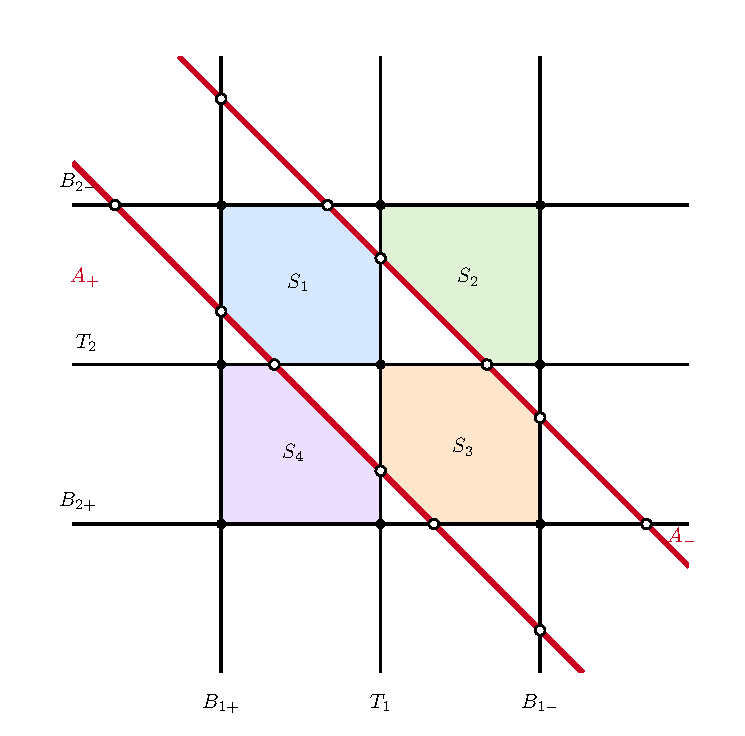
\includegraphics{summation_singular_lines.pdf}
    \caption{完整 $\Omega_N$ 积分族在 $x_1$-$x_2$ 平面上的超平面排列。}
\end{figure}

\subsection{xq 表示中的 $\mathcal{I}_1$ 积分族}

利用上文的 t→x 变换结果，$(++)$ 构型的 $\tau$ 积分已化为 $x$ 积分和动量积分的形式。两项共享公因子 $1/(k_1+k_2+x_1+x_2)$，但第二分母不同。由于积分为两项之和，我们可分别处理每一项，无需考虑同时包含两个第二分母的积分族。定义 \textbf{xq 积分族}
\begin{equation}
    \boxed{\mathcal{I}_1[a_1,a_2,a_3,a_4,a_5,a_6]=\int_0^{\infty}dx_1dx_2\int\frac{d^d\boldsymbol{q}}{(2\pi)^d}\frac{(x_1x_2)^\epsilon}{D_1^{a_1}D_2^{a_2}D_3^{a_3}D_4^{a_4}D_5^{a_5}D_6^{a_6}}},
    \label{xqfamily}
\end{equation}
其中分母为
\begin{align}
    D_1=x_1,\qquad D_2=x_2,\qquad D_3=k_1+k_2+x_1+x_2,\notag\\
    D_4=k_1+x_1+q_1+q_2,\qquad D_5=q_1,\qquad D_6=q_2.
\end{align}
指数 $a_1,\dots,a_6$ 为整数（或解析延拓）；仅有的非 $a_i$ 指数是 $x_1,x_2$ 上的维度正规化参数 $\epsilon$ 和测度 $d^d\boldsymbol{q}/(2\pi)^d$ 中的时空维度 $d$。

\textbf{分离项说明。} 在被积函数层面，$(++)$ 求和中的两项——以及四种 SK 构型的类似情形——分别产生含 $D_4=k_1+x_1+q_1+q_2$ 和 $D_4'=k_2+x_2+q_1+q_2$ 的分母。由于二者从不出现在同一求和项的乘积中，我们无需考虑同时包含 $D_4$ 和 $D_4'$ 的积分族。仅含 $D_4$ 的族 (\ref{xqfamily})（以及对称的 $D_4\to D_4'$ 版本）已足够。

对这个具体族，若暂时把动量模长 $q_1,q_2$ 当作参数，只看 $x_1,x_2$ 平面，则被积函数中参与 $x$-apart 的四个因子为
\[
\frac{1}{D_1^{a_1}}\frac{1}{D_2^{a_2}}\frac{1}{D_3^{a_3}}\frac{1}{D_4^{a_4}}.
\]
这里的四因子不是抽象地从 t→x 变换直接得到，而是由上面选定的 $(++)$ 分离项积分族给出。若用 $D_4-D_1-D_5-D_6=k_1$ 降低 $D_4$ 的幂次，原本只在动量测度或传播子中出现的 $D_5,D_6$ 会进入同一个积分表示。它们的奇性位于动量积分的端点或阈值附近，不能和 $x_1,x_2$ 的端点问题混为一谈；因此，冻结动量后做的 $x$-apart 只是代数重写，后续动量 IBP 仍需单独检查边界项。

\subsection{xq 表示中的 wavefunction coefficient}

kinematic-flow 文献通常直接组织 wavefunction coefficient，而不是晚时 correlator 本身。下面把 two-site one-loop bubble 公式统一改写成本项目记号：两个顶点外部能量和仍记为 $k_1,k_2$，两条内线能量分别记为 $q_1$ 和 $q_2$。

由式 (\ref{wfpropagators}) 的 wavefunction Feynman 规则可得 flat-space bubble integrand \cite{Hang:2024frw}
\begin{align}
    \widetilde{\psi}^{\rm flat,bub}_{(2,1)}
    &=
    i^2\int_{-\infty}^{0}d\tau_1d\tau_2\,
    K(k_1;\tau_1)K(k_2;\tau_2)
    G(q_1;\tau_1,\tau_2)
    G(q_2;\tau_2,\tau_1)\notag\\
    &=
    \frac{2(k_1+k_2+q_1+q_2)}
    {(k_1+k_2)
     (k_1+k_2+2q_1)
     (k_1+k_2+2q_2)
     (k_1+q_1+q_2)
     (k_2+q_1+q_2)}.
    \label{flatwfbubble}
\end{align}
这个公式是和 kinematic flow 对比时最有用的起点：它已经把所有 bulk-time ordering 求和做完，剩下的是能量变量上的有理函数。对 power-law FRW 或 dS 极限中的同一 wavefunction integrand，只需按式 (\ref{wfenergyshift}) 做顶点能量 shift：
\begin{equation}
    k_1\to k_1+x_1,\qquad k_2\to k_2+x_2.
\end{equation}
在忽略整体归一化后，得到
\begin{equation}
    \psi^{\rm FRW,bub}_{(2,1)}
    =
    \int_0^\infty dx_1dx_2\,(x_1x_2)^\epsilon
    \left[
    \frac{4q_1\,q_2}
    {D^{\rm wf}_3D^{\rm wf}_4D^{\rm wf}_5}
    \left(\frac{1}{D^{\rm wf}_6}+\frac{1}{D^{\rm wf}_7}\right)
    \right],
    \label{frwwfbubble}
\end{equation}
其中 wavefunction 超平面分母定义为
\begin{align}
    D^{\rm wf}_1&=x_1,\qquad
    D^{\rm wf}_2=x_2,\notag\\
    D^{\rm wf}_3&=x_1+x_2+k_1+k_2,\notag\\
    D^{\rm wf}_4&=x_1+k_1+q_1+q_2,\notag\\
    D^{\rm wf}_5&=x_2+k_2+q_1+q_2,\notag\\
    D^{\rm wf}_6&=x_1+x_2+k_1+k_2+2q_1,\notag\\
    D^{\rm wf}_7&=x_1+x_2+k_1+k_2+2q_2.
    \label{wfbubbledenoms}
\end{align}
这里 $D^{\rm wf}_1,D^{\rm wf}_2$ 是 twist 分母，其余 $D^{\rm wf}_i$ 是相对奇性分母。与式 (\ref{xqfamily}) 的 correlator 分离项相比，wavefunction 公式 (\ref{frwwfbubble}) 同时保留了两个 bubble 内线对应的相对分母 $D^{\rm wf}_6,D^{\rm wf}_7$，并且它们通过括号中的和出现；而当前 SK correlator 的 $\mathcal{I}_1$ 是选定某个 time-ordering 分离项后得到的单项积分族。因此，kinematic-flow 的 master integral basis 可以作为超平面和 DE 的参考，但不能直接等同于本项目的 massless correlator 约化族。

\textbf{与超平面排列和临界点方程的关系。} 固定 $q_1,q_2$ 后，每个分母方程 $D^{\rm wf}_i=0$ 在 $x_1,x_2$ 平面上给出一条直线。主积分个数可以从这些直线围出的有限区域读取，也可以从对应 master function 的有限孤立临界点读取；这两个读法在通用参数下给出同一个数。为避免打断正文推导，具体的通分例子、临界方程和“为什么无穷远区域不算”的解释统一放在附录 \ref{app:geometry-critical-points}。

\begin{table}[htbp]
    \centering
    \caption{Conformal wavefunction 与本项目 correlator 函数族的差别。}
    \begin{tabular}{p{0.25\linewidth}p{0.32\linewidth}p{0.32\linewidth}}
        \toprule
        项目 & conformal wavefunction & 本项目 correlator / massless bubble \\
        \midrule
        目标对象 & $\psi_m$，由 $\Psi[\phi]$ 的指数展开定义 & 晚时 correlator，使用 SK 闭时路径求和 \\
        bulk-to-boundary & $K(E;\tau)=e^{iE\tau}$ & $D_\pm(k;\tau)=e^{\pm ik\tau}/(2k)$；massless 时还含 $(1\mp ik\tau)/(2k^3)$ \\
        bulk propagator & 含边界项 $-e^{iE(\tau+\tau')}$ 的 $G(E;\tau,\tau')$ & SK 的 $D_{\pm\pm},D_{\pm\mp}$，无 wavefunction Dirichlet 边界项 \\
        $x$ 变量来源 & $k_v\to k_v+x_v$ 的 vertex energy shift & 对每个 tq 展开项做指数积分表示，得到 $x_1,x_2$ 与 time-ordering 分母 \\
        two-site bubble 分母 & $D^{\rm wf}_3,\dots,D^{\rm wf}_7$ 同属 wavefunction 超平面排列 & $\mathcal{I}_1$ 选取 $D_1,\dots,D_6$ 的单个分离项族 \\
        kinematic flow 适用性 & 文献已建立 conformal wavefunction / loop integrand 规则 & 只能作为对照；massless 多项式因子和 SK 求和需逐项核对 \\
        \bottomrule
    \end{tabular}
\end{table}

另一个互补表述是在 loop integrand 层面用 marked tubing graph 描述 master integrals 和微分方程奇性 \cite{Baumann:2024loop}。例如 bubble 的 flat-space wavefunction 可拆成两个 tubing 贡献，其分母分别含 $k_1+k_2+2q_1$ 与 $k_1+k_2+2q_2$；这正对应式 (\ref{frwwfbubble}) 中 $D^{\rm wf}_6,D^{\rm wf}_7$ 的两项。后续若要把 kinematic flow 用于本项目，应先把每个 SK/time-ordering 分离项映射到类似的能量超平面，再比较 DE 的 alphabet。

\newpage
% ============================================================
\section{xq 约化关系}
% ============================================================

本章推导 xq 积分族 $\mathcal{I}_1$ 的约化恒等式。关系分两类：由分母 $D_1,\dots,D_6$ 之间的线性相关性产生的 apart 等式，以及由 $x_1,x_2$ 和动量变量产生的分部积分（IBP）恒等式。下文先固定采用 (\ref{xqfamily}) 中的 $(x_1x_2)^\epsilon$ 表示；若某个物理情形的 t→x 变换本身不需要该正规化，仍可把它理解为 IBP 边界项的解析调节参数，最后再取相应极限。

\subsection{代数 apart 约化}

六个分母 $D_1,\dots,D_6$ 是四个独立变量 $(x_1,x_2,q_1,q_2)$ 的函数，因此它们之间存在线性关系。由定义可得
\begin{align}
    D_3-D_1-D_2 &= k_1+k_2, \label{apart1}\\
    D_4-D_1-D_5-D_6 &= k_1, \label{apart2}\\
    D_3-D_2-D_4+D_5+D_6 &= k_2. \label{apart3}
\end{align}
这三个关系并非独立（第三个可由前两个导出）；以前两个为基。

\textbf{apart 无法消除任何分母的数学原因。} 考虑 (\ref{apart1})：$D_3 = D_1+D_2+(k_1+k_2)$。将其用于被积函数层面的约化时，
\begin{align}
    \mathcal{I}_1 = \frac{1}{k_1+k_2}\Bigl\{\mathcal{I}_1[a_3-1]-\mathcal{I}_1[a_1-1]-\mathcal{I}_1[a_2-1]\Bigr\}.
\end{align}
RHS 中 $\mathcal{I}_1[a_1-1]$ 这一项：$a_1$ 降低了 1，但其他五个指数（$a_2,a_3,a_4,a_5,a_6$）均\textbf{保持原值不变}。这意味着无论迭代多少次，右边始终存在一项，其 $a_2,a_3,\dots$ 保持原始正幂次——仅 $a_1$ 被逐次降低。同理，$\mathcal{I}_1[a_2-1]$ 项中 $a_1$ 不变。

关系 (\ref{apart2}) 和 (\ref{apart3}) 的处境相同——每个关系都涉及 $D_1$ 或 $D_2$，且都包含一个"仅移位 $a_1$（或 $a_2$）而其他指数不变"的项。通过消去 $D_1,D_2$ 组合这三个关系，得到的仍是 (\ref{apart3})，因此\textbf{不存在不涉及 $x_1,x_2$ 的分母线性关系}。

\textbf{结论：} 既然全部三个线性关系都涉及 $x_1$ 或 $x_2$，且每个关系的 RHS 都有"仅 $x_i$ 幂次改变而其他分母幂次不变"的项，那么 apart \textbf{不仅消不掉 $D_1,D_2$，也消不掉其他任何分母}——$D_3,D_4,D_5,D_6$ 同样因为在每次移位中总有一项保持它们的原始正幂次而无法被消除。六个分母中没有任何一个可以通过 apart 约化到零，所有分母的消除必须依赖 IBP。

尽管如此，apart 等式仍有实用价值：当需要将某一分母的正幂次降低时（例如从 $a_3=2$ 降到 $a_3=1$），apart 提供无 $\epsilon$ 依赖的移位。下面列出三条 apart 移位关系的显式及各关系可作用的 sector 条件。

利用 (\ref{apart1})，当 $a_1,a_2,a_3>0$ 时：
\begin{align}
    \mathcal{I}_1={}&\frac{1}{k_1+k_2}\Bigl\{
        \mathcal{I}_1[a_3-1]-\mathcal{I}_1[a_1-1]-\mathcal{I}_1[a_2-1]\Bigr\}.
\end{align}
利用 (\ref{apart2})，当 $a_1,a_4,a_5,a_6>0$ 时：
\begin{align}
    \mathcal{I}_1={}&\frac{1}{k_1}\Bigl\{
        \mathcal{I}_1[a_4-1]-\mathcal{I}_1[a_1-1]
        -\mathcal{I}_1[a_5-1]-\mathcal{I}_1[a_6-1]\Bigr\}.
\end{align}
利用 (\ref{apart3})，当 $a_2,a_3,a_4,a_5,a_6>0$ 时：
\begin{align}
    \mathcal{I}_1={}&\frac{1}{k_2}\Bigl\{
        \mathcal{I}_1[a_3-1]-\mathcal{I}_1[a_2-1]-\mathcal{I}_1[a_4-1]
        +\mathcal{I}_1[a_5-1]+\mathcal{I}_1[a_6-1]\Bigr\}.
\end{align}

\subsubsection{x-apart 引入的新分母与动量边界项}

当在 apart 中将 $q_1,q_2$ 视为冻结参量时，前两条 apart 等式会引入 $D_5=q_1$ 和 $D_6=q_2$ 作为新分母。例如利用 (\ref{apart2}) 将 $D_4$ 的幂次降低时，RHS 出现含 $D_5,D_6$ 的项。这些 $D_5,D_6$ 的零点对应内线模长的奇性，动量积分还另有无穷远边界；因此，在随后的动量 IBP 中，不能把它们当成普通的 $x$-apart 可消因子，必须单独检查边界项 $\int d^d\boldsymbol{q}\,\partial_{q^\mu}(\cdots)$。

此外，$D_5$ 与 $D_6$ 之间也存在线性关系（二者通过 $k_3$ 关联：$D_6^2 = D_5^2 + k_3^2 + 2\boldsymbol{q}\cdot\boldsymbol{k}_3$），但由于该关系非线性且依赖于 $\boldsymbol{q}$ 的角度变量，无法直接用于 apart 消去分母。在 IBP 层面，$\mathcal{O}_{q_1}$ 和 $\mathcal{O}_{q_2}$ 算子提供了 $D_5,D_6$ 指数移位的关系（见 §3.2），结合 $\mathcal{O}_\perp$ 可得到不含奇组合的封闭形式。

\subsubsection{apart 的两种处理路径}

既然 apart 无法消除任何分母，在实际计算中有两种策略来处理 apart 等式：

\begin{enumerate}
    \item \textbf{直接与 IBP 一同扔给约化程序。} 将 apart 等式与 IBP 关系作为同一组线性方程输入 Kira 等约化工具，由程序统一求解。这种方式的优点是不需要人工干预 apart 化简，缺点是没有利用 apart 无 $\epsilon$ 依赖的特性来简化系统。

    \item \textbf{先约定幂次零点，用 apart 确定唯一表示，再做 IBP。} 选定一个幂次零点（例如所有 $a_i=0$ 或某个特定参考幂次点）。apart 等式只能先消去一部分代数冗余，把积分改写到约定的关于 apart 的标准形式。然后在此标准形式上建立 IBP 关系进行约化。在实践中，通常取零点为所有分母的幂次均非正，并约定在 apart 等式下通过移位使得带正幂次的分母种类数达到极小。
\end{enumerate}

两种路径各有适用场景：路径 1 适合快速验证和小规模系统；路径 2 适合对最终 DE 系统进行系统化构造，因其能够显著压缩输入 IBP 的关系数量。

\begin{proofbox}
\textbf{主积分个数。} 对单独的 $x$ 积分，暂时冻结动量变量 $q_1,q_2$ 后，图 2 中 $D_1=0,D_2=0,D_3=0,D_4=0$ 四条直线围出两个有限三角形区域，因此该 $x$-sector 有 2 个主积分。等价的临界点方程也给出两个有限孤立解；详细推导见附录 \ref{app:geometry-critical-points}。

\begin{minipage}{\linewidth}
    \centering
    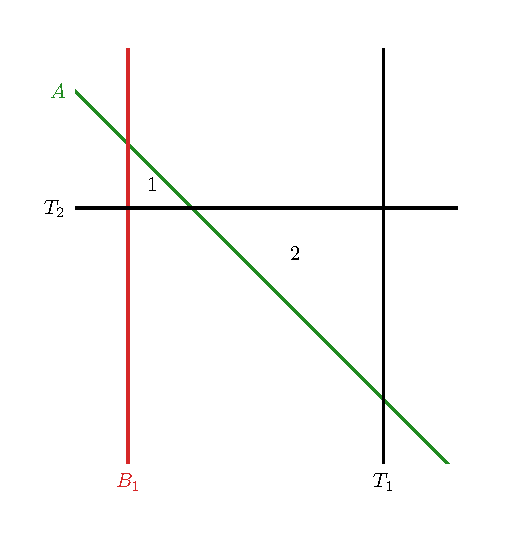
\includegraphics[scale=0.6]{separated_family_singular_lines.pdf}
    {\small\textbf{图 2}：分离 $\mathcal{I}_1$ 族的超平面排列。四条线 $D_1=0$, $D_2=0$, $D_3=0$, $D_4=0$ 在 $x_1$-$x_2$ 平面上围出两个有限三角形区域；它们对应该 $x$-sector 的两个主积分。}
\end{minipage}
\end{proofbox}

\subsection{IBP 关系}

\textbf{记号。} 以下 IBP 恒等式中采用简洁记法：无参数的 $\mathcal{I}_1$ 表示当前 sector $[a_1,\dots,a_6]$；仅显式写出相对当前 sector 有移位的指数，例如 $\mathcal{I}_1[a_4+1,a_5-1]$ 表示 $[a_1,a_2,a_3,a_4+1,a_5-1,a_6]$。

对动量 IBP 引入微分算子
\begin{equation}
    \mathcal{O}_{q_1}\equiv q^\mu\partial_{q^\mu},\qquad 
    \mathcal{O}_{q_2}\equiv (q^\mu+k_3^\mu)\partial_{q^\mu},
\end{equation}
基本作用为
\begin{align}
    \mathcal{O}_{q_1}q_1=q_1,&\qquad \mathcal{O}_{q_1}q_2=\frac{1}{2}q_2^{-1}(q_1^2+q_2^2-k_3^2),\\
    \mathcal{O}_{q_2}q_2=q_2,&\qquad \mathcal{O}_{q_2}q_1=\frac{1}{2}q_1^{-1}(q_1^2+q_2^2-k_3^2).
\end{align}
对一般函数 $F(q_1,q_2)$，
\begin{equation}
    \mathcal{O}_{\alpha}F(q_1,q_2)=(\mathcal{O}_{\alpha}q_1)\,\partial_{q_1}F+(\mathcal{O}_{\alpha}q_2)\,\partial_{q_2}F,\qquad \alpha=q_1,q_2.
\end{equation}

$\mathcal{O}_{q_1}$ IBP 关系（来自 $\partial_{q^\mu}(q^\mu\cdots)=0$）为
\begin{align}
    0={}&\Bigl(d-a_5-\frac{a_6}{2}\Bigr)\mathcal{I}_1
        -\frac{a_6}{2}\mathcal{I}_1[a_5-2,a_6+2]\notag\\
    &+\frac{a_6 k_3^2}{2}\mathcal{I}_1[a_6+2]
        -\frac{a_4}{2}\mathcal{I}_1[a_4+1,a_5-2,a_6+1]\notag\\
    &-a_4\mathcal{I}_1[a_4+1,a_5-1]
        -\frac{a_4}{2}\mathcal{I}_1[a_4+1,a_6-1]\notag\\
    &+\frac{a_4 k_3^2}{2}\mathcal{I}_1[a_4+1,a_6+1].
    \label{IBPq1}
\end{align}
$\mathcal{O}_{q_2}$ IBP 关系（来自 $\partial_{q^\mu}((q^\mu+k_3^\mu)\cdots)=0$）为
\begin{align}
    0={}&\Bigl(d-\frac{a_5}{2}-a_6\Bigr)\mathcal{I}_1
        -\frac{a_5}{2}\mathcal{I}_1[a_5+2,a_6-2]\notag\\
    &+\frac{a_5 k_3^2}{2}\mathcal{I}_1[a_5+2]
        -\frac{a_4}{2}\mathcal{I}_1[a_4+1,a_5-1]\notag\\
    &-a_4\mathcal{I}_1[a_4+1,a_6-1]
        -\frac{a_4}{2}\mathcal{I}_1[a_4+1,a_5+1,a_6-2]\notag\\
    &+\frac{a_4 k_3^2}{2}\mathcal{I}_1[a_4+1,a_5+1].
    \label{IBPq2}
\end{align}

对 $x_1$ 和 $x_2$ 变量，边界 IBP 关系（来自 $\int dx_1\,\partial_{x_1}(\cdots)=0$ 等）为：
\begin{align}
    0={}&(1+\epsilon-a_1)\mathcal{I}_1
        -a_3\,\mathcal{I}_1[a_1-1,a_3+1]
        -a_4\,\mathcal{I}_1[a_1-1,a_4+1],\\
    0={}&(1+\epsilon-a_2)\mathcal{I}_1
        -a_3\,\mathcal{I}_1[a_2-1,a_3+1].
\end{align}

最后，施加维度正规化下无标度动量积分为零的条件。当 $a_4=0$ 且 $a_5=0$ 或 $a_6=0$ 时，积分分解为 $x$ 积分乘以无标度动量积分，因此
\begin{equation}
    \mathcal{I}_1[a_4=0,a_5=0]=\mathcal{I}_1[a_4=0,a_6=0]=0.
\end{equation}
初步 Kira 运行表明完整 $\mathcal{I}_1$ 族约有 $8$ 个主积分，但该数字有待确认。


\newpage
% ============================================================
\section{xq 微分方程}
% ============================================================

\textcolor{red}{待完成：$\mathcal{I}_1$ 族关于外部标度 $k_1,k_2,k_3$ 的完整 $\epsilon$-形式与 canonical basis。}

xq 积分族 $\mathcal{I}_1$ 依赖于外部标度 $k_1,k_2,k_3$。对这些标度求导会把分母指数移位，因此 DE 系统可统一写成
\begin{align}
    \frac{\partial}{\partial k_r}\vec{\mathcal{I}}_1
    =A_r(a,d,\epsilon;k)\,\vec{\mathcal{I}}_1,\qquad r=1,2,3,
\end{align}
其中 $\vec{\mathcal{I}}_1$ 表示选定的积分向量，$A_r$ 由 IBP 约化后的移位积分系数给出。标度关系（Euler 算子）为
\begin{equation}
    \Bigl(\sum_{r=1}^{3} k_r\frac{\partial}{\partial k_r}\Bigr)\mathcal{I}_1
    =\bigl(d-a_3-a_4-a_5-a_6\bigr)\mathcal{I}_1.
\end{equation}
$x_1,x_2$ 积分通过 $\epsilon$ 参数贡献额外的质量量纲，这将在 $\epsilon$ 正规化方案最终确定后计入。

\textcolor{red}{待完成：DE 系统 $\epsilon$-形式构造。Canonical basis 选取。迭代积分求解。}

\newpage
% ============================================================
\section{tq IBP 关系}
% ============================================================

现回到 tq 表示，直接在共形时间中推导 IBP 关系，无需转换为能量变量。其优点是不需 t→x 变换；代价是必须小心处理 Heaviside 阶梯函数在 IBP 中的行为。

\subsection{$(++)$ 情形：tq 积分族}

\begin{center}
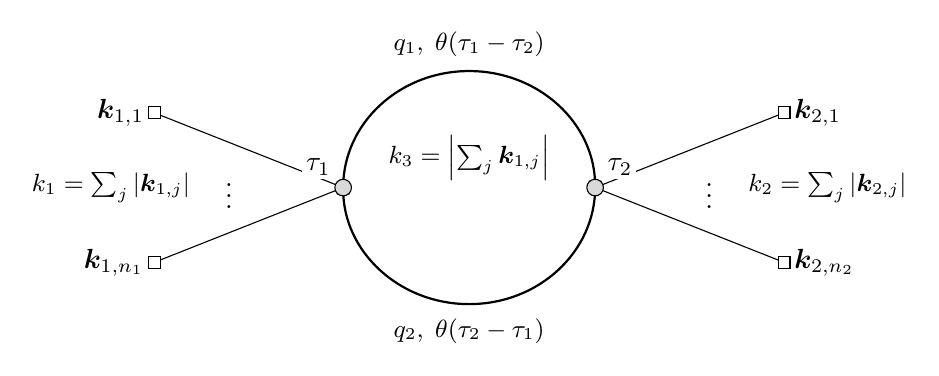
\begin{tikzpicture}[scale=1.0, every node/.style={inner sep=1.5pt}]
  \coordinate (vL) at (0,0);
  \coordinate (vR) at (3.2,0);
  \coordinate (lU) at (-2.4,0.95);
  \coordinate (lD) at (-2.4,-0.95);
  \coordinate (rU) at (5.6,0.95);
  \coordinate (rD) at (5.6,-0.95);
  \draw (vL) -- (lU) node[left=2pt] {$\boldsymbol{k}_{1,1}$};
  \draw (vL) -- (lD) node[left=2pt] {$\boldsymbol{k}_{1,n_1}$};
  \draw (vR) -- (rU) node[right=2pt] {$\boldsymbol{k}_{2,1}$};
  \draw (vR) -- (rD) node[right=2pt] {$\boldsymbol{k}_{2,n_2}$};
  \node[fill=white,inner sep=1pt] at (-1.45,0) {$\vdots$};
  \node[fill=white,inner sep=1pt] at (4.65,0) {$\vdots$};
  \draw[->,thick] (vL) arc[start angle=180,end angle=0,x radius=1.6,y radius=1.48];
  \draw[->,thick] (vR) arc[start angle=0,end angle=-180,x radius=1.6,y radius=1.48];
  \node[fill=white] at (1.6,1.82) {\small $q_1,\;\theta(\tau_1-\tau_2)$};
  \node[fill=white] at (1.6,-1.82) {\small $q_2,\;\theta(\tau_2-\tau_1)$};
  \node[fill=white] at (1.6,0.38) {\small $k_3=\left|\sum_j\boldsymbol{k}_{1,j}\right|$};
  \node[fill=white] at (-2.95,0) {\small $k_1=\sum_j|\boldsymbol{k}_{1,j}|$};
  \node[fill=white] at (6.15,0) {\small $k_2=\sum_j|\boldsymbol{k}_{2,j}|$};
  \filldraw[fill=gray!30,draw=black] (vL) circle (3pt);
  \filldraw[fill=gray!30,draw=black] (vR) circle (3pt);
  \node[fill=white,anchor=south east] at (-0.10,0.10) {$\tau_1$};
  \node[fill=white,anchor=south west] at (3.30,0.10) {$\tau_2$};
  \filldraw[fill=white,draw=black] ($(lU)+(-0.075,0.075)$) rectangle ++(0.15,-0.15);
  \filldraw[fill=white,draw=black] ($(lD)+(-0.075,0.075)$) rectangle ++(0.15,-0.15);
  \filldraw[fill=white,draw=black] ($(rU)+(-0.075,0.075)$) rectangle ++(0.15,-0.15);
  \filldraw[fill=white,draw=black] ($(rD)+(-0.075,0.075)$) rectangle ++(0.15,-0.15);
\end{tikzpicture}
\end{center}

Bubble 图的 $(++)$ 贡献在 family tree 化简后为
\begin{align}
    \mathcal{T}^{(1)}_{++}&\propto\int_{-\infty}^0d\tau_1d\tau_2\,(-\tau_1)^{a_1}(-\tau_2)^{a_2}
    \int\frac{d^d\boldsymbol{q}}{(2\pi)^d}
    \Bigl[e^{i(k_1-q_1-q_2)\tau_1}e^{i(k_2+q_1+q_2)\tau_2}\theta(\tau_1-\tau_2)\notag\\
    &\qquad+e^{i(k_1+q_1+q_2)\tau_1}e^{i(k_2-q_1-q_2)\tau_2}\theta(\tau_2-\tau_1)\Bigr]
    \frac{1}{q_1^{a_3}}\frac{1}{q_2^{a_4}}.
    \label{ppcase}
\end{align}
（与第 2 章的 xq 表示相比，此处的 $a_1,a_2$ 为分子上的时间幂次指数；动量指数为 $a_3,a_4$。粗略地说，先积掉 $\tau$ 后，$\tau$ 的分子幂次会变成能量分母的幂次，所以 tq 表示中不把 $\tau$ 幂次写在分母上。）

为实施 IBP，需使边界项消失。晚时 $\tau\to0$ 处要求相应时间幂次的实部足够大；若某个具体物理项需要额外解析调节，可在使用时把对应的 $a_i$ 取成带调节量的值。下面的 tq 函数族定义不默认额外写入这个调节量。早时处使用标准的 $i\epsilon$ 围道延拓。

\begin{equation}
    \boxed{
    \begin{gathered}
    \text{tq 族标号：}\quad
    1\leftrightarrow q_1=|\boldsymbol{q}|,\qquad
    2\leftrightarrow q_2=|\boldsymbol{q}+\boldsymbol{k}_3|,\\
    +\leftrightarrow \theta(\tau_1-\tau_2),\ e^{-i|\cdot|(\tau_1-\tau_2)},\qquad
    -\leftrightarrow \theta(\tau_2-\tau_1),\ e^{+i|\cdot|(\tau_1-\tau_2)}.
    \end{gathered}}
\end{equation}
两个传播子是否存在已经由后面的动量幂次槽位 $a_3,a_4$ 表示，因此本节不再用 $11$ 作为函数族下标。A 类两 Heaviside 合并处理记为 $\mathcal{I}_{\pm}$；B 类单通道处理记为 $\mathcal{I}_{\sigma_1,\sigma_2}$，其中 $\sigma_i=\pm$ 是第 $i$ 条传播子的 time-ordering 符号。

先把 bubble 中实际出现的两项写成
\begin{align}
    \Phi_{+}&=e^{i(k_1-q_1-q_2)\tau_1
    +i(k_2+q_1+q_2)\tau_2}\theta(\tau_1-\tau_2),\\
    \Phi_{-}&=e^{i(k_1+q_1+q_2)\tau_1
    +i(k_2-q_1-q_2)\tau_2}\theta(\tau_2-\tau_1).
\end{align}
若暂时不利用 massless 指数核的简化，也可以给每条传播子的两个端点各自放一个导数计数。Bubble 中这只是一个过渡性的 naive 写法，不作为后续 IBP 的正式函数族：
\begin{equation}
\begin{aligned}
    &\mathcal{I}_{\pm}^{\mathrm{naive}}[\{n_{1,1}n_{1,2};n_{2,1}n_{2,2}\},a_1,a_2,a_3,a_4]\\
    &\quad=\int d\tau_1d\tau_2\,(-\tau_1)^{a_1}(-\tau_2)^{a_2}
    \int\frac{d^d\boldsymbol{q}}{(2\pi)^d}
    e^{ik_1\tau_1+ik_2\tau_2}\frac{1}{q_1^{a_3}q_2^{a_4}}\\
    &\qquad\times\Bigl[
    \partial_{\tau_1}^{n_{1,1}}\partial_{\tau_2}^{n_{1,2}}e^{-iq_1(\tau_1-\tau_2)}
    \,\partial_{\tau_1}^{n_{2,1}}\partial_{\tau_2}^{n_{2,2}}e^{-iq_2(\tau_1-\tau_2)}
    \theta(\tau_1-\tau_2)
    \Bigr.\\
    &\qquad\qquad\Bigl.
    +\partial_{\tau_1}^{n_{1,1}}\partial_{\tau_2}^{n_{1,2}}e^{+iq_1(\tau_1-\tau_2)}
    \,\partial_{\tau_1}^{n_{2,1}}\partial_{\tau_2}^{n_{2,2}}e^{+iq_2(\tau_1-\tau_2)}
    \theta(\tau_2-\tau_1)
    \Bigr].
\end{aligned}
\end{equation}
这里第一对 $n_{1,1},n_{1,2}$ 属于 $q_1$ 传播子，第二对 $n_{2,1},n_{2,2}$ 属于 $q_2$ 传播子。这个 naive 标签只用来说明端点导数从哪里来；A 类真正用于 IBP 的简化标签在下一小节重新定义。

对时间 IBP，Heaviside 函数的导数会产生一个子拓扑，其中两个时间变量塌缩为单积分。该族不能表示成双传播子族的某些幂次取零，因此在基础定义处单独列出：
\begin{equation}
    \mathcal{I}_{\delta}[a_1,a_2,a_3,a_4]=\int_{-\infty}^{0}d\tau\,(-\tau)^{a_1+a_2}
    e^{i(k_1+k_2)\tau}\int\frac{d^d\boldsymbol{q}}{(2\pi)^d}\frac{1}{q_1^{a_3}q_2^{a_4}}.
\end{equation}

\subsection{A 类：两项 Heaviside 合并处理}

先看 A 类：无质量传播子中，把同一对顶点之间的两个 time-ordering 项合并处理。若两个顶点之间有多条传播子，例如圈图中的若干条内线，它们的 Heaviside 因子不是 $2^N$ 个独立项。原因很简单：同一对时间只有两个互斥区域，
\begin{equation}
    \tau_1>\tau_2,\qquad \tau_2>\tau_1.
\end{equation}
混合项中若同时出现 $\theta(\tau_1-\tau_2)$ 和 $\theta(\tau_2-\tau_1)$，其支撑为空；除去端点测度零的 pinched 位置，只剩“所有传播子都走第一项”和“所有传播子都走第二项”两类。因此同一对顶点之间的多条传播子可以合并成一对 Heaviside 分支，而不是给每条传播子保留一对独立的 time-ordering 标签。

这一点还会进一步简化端点导数标签。对每一对顶点之间的整束传播子，先记一对端点标签
\begin{equation}
    \{n_{i,1}n_{i,2}\},
\end{equation}
其中 $i$ 标记顶点对，而不是单条传播子。当前 bubble 只有一对顶点，因此下面省略这个 $i$。Massless 指数核满足
\begin{equation}
    \partial_{\tau_1}e^{\mp iq(\tau_1-\tau_2)}
    =
    -\partial_{\tau_2}e^{\mp iq(\tau_1-\tau_2)},\qquad
    \partial_{\tau_1}\partial_{\tau_2}e^{\mp iq(\tau_1-\tau_2)}
    =
    q^2 e^{\mp iq(\tau_1-\tau_2)}.
\end{equation}
所以 $\{10\}$ 与 $\{01\}$ 不是两个独立方向；它们只差一个负号。$\{11\}$ 也不是新函数族，而是给出一个 $q^2$ 因子，等价于降低对应传播子的动量幂次。对 bubble 的两条内线具体写为
\begin{equation}
    \{10\}=-\{01\},\qquad
    \{11\}=q_1^2\{00\}\ \text{或}\ q_2^2\{00\},
\end{equation}
其中 $q_1^2$ 对应 $a_3\to a_3-2$，$q_2^2$ 对应 $a_4\to a_4-2$。

因此 A 类可以不用 naive 的多端点标签作为最终 notation。对每一对顶点记一个指标 $n_i$，其中 $i$ 标记这对顶点。当前 bubble 只有这一对顶点，所以函数族第一槽就是这个 $n_i$；$n_i=0,1$ 分别表示两项 Heaviside 组合的对称或反对称部分：
\begin{equation}
    \begin{aligned}
    \mathcal{I}_{\pm}[\{0\},a_1,a_2,a_3,a_4]
    =
    &\int d\tau_1d\tau_2\,(-\tau_1)^{a_1}(-\tau_2)^{a_2}
    \int\frac{d^d\boldsymbol{q}}{(2\pi)^d}
    \frac{\Phi_++\Phi_-}{q_1^{a_3}q_2^{a_4}},\\
    \mathcal{I}_{\pm}[\{1\},a_1,a_2,a_3,a_4]
    =
    &\int d\tau_1d\tau_2\,(-\tau_1)^{a_1}(-\tau_2)^{a_2}
    \int\frac{d^d\boldsymbol{q}}{(2\pi)^d}
    \frac{-\Phi_++\Phi_-}{q_1^{a_3}q_2^{a_4}}.
    \end{aligned}
\end{equation}
下面所有 A 类 bubble 公式都按这个最终约定书写；第一槽的 $\{0\}$ 或 $\{1\}$ 就是这一对顶点的 $\{n_i\}$。若图中有多对顶点，则每一对顶点各有自己的 $n_i$。在 massive Hankel 情形中，同一端点导数会把 $h_{\nu}(n;q_i\tau_a)$ 提升到新的 Hankel building block；两端导数通常仍是独立对象。Massless 指数核把这些对象压缩成上面的 $n_i=0,1$ 两类，这是 A 相对 massive 两 theta 处理的额外简化。若后续要把无质量族和有质量 Hankel 族放在同一个框架中处理，A 类两 theta 合并方式更容易和 massive 的两 theta/Hankel building block 组织方式对齐；若只处理纯无质量系统，B 类单 theta 或积掉时间后的表示通常更轻。

时间 IBP 现在按这个最终 notation 书写。由于
\begin{equation}
    \partial_{\tau_1}(\Phi_++\Phi_-)
    =
    ik_1(\Phi_++\Phi_-)+i(q_1+q_2)(-\Phi_++\Phi_-),
\end{equation}
且两个 $\delta(\tau_1-\tau_2)$ 项在对称组合中相消，$\tau_1$-IBP 给出
\begin{align}
    0={}&-a_1\mathcal{I}_{\pm}[\{0\},a_1-1,a_2,a_3,a_4]
    +ik_1\mathcal{I}_{\pm}[\{0\},a_1,a_2,a_3,a_4]\notag\\
    &+i\mathcal{I}_{\pm}[\{1\},a_1,a_2,a_3-1,a_4]
    +i\mathcal{I}_{\pm}[\{1\},a_1,a_2,a_3,a_4-1].
    \label{tau1IBPnew}
\end{align}
同理，
\begin{align}
    0={}&-a_2\mathcal{I}_{\pm}[\{0\},a_1,a_2-1,a_3,a_4]
    +ik_2\mathcal{I}_{\pm}[\{0\},a_1,a_2,a_3,a_4]\notag\\
    &-i\mathcal{I}_{\pm}[\{1\},a_1,a_2,a_3-1,a_4]
    -i\mathcal{I}_{\pm}[\{1\},a_1,a_2,a_3,a_4-1].
    \label{tau2IBPnew}
\end{align}
这里两条 IBP 仍然单独保留；不把它们相加压缩，因为单独方程在后续构造 DE 和检查子拓扑项时更有信息。

对动量 IBP，标准算子微分指数中的 $q_1+q_2$ 时会把 $n_i=0$ 切换成 $n_i=1$。
$\mathcal{O}_{q_1}=q^\mu\partial_{q^\mu}$ IBP 给出
\begin{align}
    0={}&\Bigl(d-a_3-\frac{a_4}{2}\Bigr)\mathcal{I}_{\pm}[\{0\},a_1,a_2,a_3,a_4]
        -\frac{a_4}{2}\mathcal{I}_{\pm}[\{0\},a_1,a_2,a_3-2,a_4+2]\notag\\
    &+\frac{a_4 k_3^2}{2}\mathcal{I}_{\pm}[\{0\},a_1,a_2,a_3,a_4+2]\notag\\
    &+i\mathcal{I}_{\pm}[\{1\},a_1+1,a_2,a_3-1,a_4]
        -i\mathcal{I}_{\pm}[\{1\},a_1,a_2+1,a_3-1,a_4]\notag\\
    &+\frac{i}{2}\mathcal{I}_{\pm}[\{1\},a_1+1,a_2,a_3-2,a_4+1]
        -\frac{i}{2}\mathcal{I}_{\pm}[\{1\},a_1,a_2+1,a_3-2,a_4+1]\notag\\
    &+\frac{i}{2}\mathcal{I}_{\pm}[\{1\},a_1+1,a_2,a_3,a_4-1]
        -\frac{i}{2}\mathcal{I}_{\pm}[\{1\},a_1,a_2+1,a_3,a_4-1]\notag\\
    &-\frac{ik_3^2}{2}\mathcal{I}_{\pm}[\{1\},a_1+1,a_2,a_3,a_4+1]
        +\frac{ik_3^2}{2}\mathcal{I}_{\pm}[\{1\},a_1,a_2+1,a_3,a_4+1].
\end{align}
$\mathcal{O}_{q_2}=(q^\mu+k_3^\mu)\partial_{q^\mu}$ IBP 给出 $a_3\leftrightarrow a_4$ 的类似关系。

也可以线性组合 $\mathcal{O}_{q_1}$ 与 $\mathcal{O}_{q_2}$ 得到不显含 $\{1\}$ 的关系；但这个关系已经组合了多个 IBP，只保留它会丢失单个动量 IBP 的信息，因此正文不把它作为主系统使用。具体公式见附录 \ref{app:tq-combined-momentum-ibp}。

\subsection{B 类：单项 Heaviside 分支处理}

B 类从一开始就不引入端点导数标签。固定每条传播子的符号 $\sigma_i=\pm$，其中 $\sigma_i=+$ 对应第一项，$\sigma_i=-$ 对应第二项。当前两点 bubble 的非零单阶梯分支有 $\sigma_1=\sigma_2$，其相位统一写为
\begin{multline}
    \Phi_{\sigma_1,\sigma_2}=
    \exp\!\left[
    i\bigl(k_1-\sigma_1 q_1-\sigma_2 q_2\bigr)\tau_1
    +i\bigl(k_2+\sigma_1 q_1+\sigma_2 q_2\bigr)\tau_2
    \right]\\
    \times\theta\!\bigl(\sigma_1(\tau_1-\tau_2)\bigr),\qquad \sigma_1=\sigma_2.
    \label{singlebranchphase}
\end{multline}
对应的 B 类积分族定义为
\begin{equation}
    \mathcal{I}_{\sigma_1,\sigma_2}[a_1,a_2,a_3,a_4]
    =
    \int d\tau_1d\tau_2\,(-\tau_1)^{a_1}(-\tau_2)^{a_2}
    \int\frac{d^d\boldsymbol{q}}{(2\pi)^d}
    \frac{\Phi_{\sigma_1,\sigma_2}}{q_1^{a_3}q_2^{a_4}}.
\end{equation}
B 的优势是方程小、可复用：$\sigma_i=+$ 与 $\sigma_i=-$ 的差别只在内线移位项和塌缩项的符号。先约化 $\mathcal{I}_{+,+}$，再通过 $\sigma_i\mapsto-\sigma_i$ 得到 $\mathcal{I}_{-,-}$，通常比先合并成 A 类更轻。具体地，单分支的 $\tau_1$-IBP 为
\begin{align}
    0={}&-a_1\mathcal{I}_{\sigma_1,\sigma_2}[a_1-1,a_2,a_3,a_4]
    +ik_1\mathcal{I}_{\sigma_1,\sigma_2}[a_1,a_2,a_3,a_4]\notag\\
    &-\sigma_1 i\,\mathcal{I}_{\sigma_1,\sigma_2}[a_1,a_2,a_3-1,a_4]
    -\sigma_2 i\,\mathcal{I}_{\sigma_1,\sigma_2}[a_1,a_2,a_3,a_4-1]
    +\sigma_1\mathcal{I}_{\delta}[a_1,a_2,a_3,a_4].
    \label{singlebranchibp}
\end{align}
$\tau_2$-IBP 也单独保留为
\begin{align}
    0={}&-a_2\mathcal{I}_{\sigma_1,\sigma_2}[a_1,a_2-1,a_3,a_4]
    +ik_2\mathcal{I}_{\sigma_1,\sigma_2}[a_1,a_2,a_3,a_4]\notag\\
    &+\sigma_1 i\,\mathcal{I}_{\sigma_1,\sigma_2}[a_1,a_2,a_3-1,a_4]
    +\sigma_2 i\,\mathcal{I}_{\sigma_1,\sigma_2}[a_1,a_2,a_3,a_4-1]
    -\sigma_1\mathcal{I}_{\delta}[a_1,a_2,a_3,a_4].
    \label{singlebranchibp2}
\end{align}
一般 $\sigma_i$ 的 $\tau_1$-IBP 已在式 (\ref{singlebranchibp}) 给出。对 $\sigma_1=\sigma_2=+$，它化为
\begin{align}
    0=-a_1\mathcal{I}_{+,+}[a_1-1,a_2,a_3,a_4]+ik_1\mathcal{I}_{+,+}[a_1,a_2,a_3,a_4]\notag\\
    -i\mathcal{I}_{+,+}[a_1,a_2,a_3-1,a_4]-i\mathcal{I}_{+,+}[a_1,a_2,a_3,a_4-1]\notag\\
    +\mathcal{I}_{\delta}[a_1,a_2,a_3,a_4],
\end{align}
而 $\tau_2$-IBP 应使用式 (\ref{singlebranchibp2})，不在这里合并成压缩关系。

塌缩子拓扑 $\mathcal{I}_{\delta}$ 满足自身的时间 IBP：
\begin{equation}
    0=-(a_1+a_2)\mathcal{I}_{\delta}[a_1-1,a_2,a_3,a_4]+i(k_1+k_2)\mathcal{I}_{\delta}[a_1,a_2,a_3,a_4],
\end{equation}
$\mathcal{I}_{\delta}$ 只依赖总时间幂次 $a_1+a_2$；上式把降幂记在第一个槽位，等价地也可记在第二个槽位。
$\mathcal{I}_{\delta}$ 的动量 IBP 由标准 $\mathcal{O}_{q_1},\mathcal{O}_{q_2}$ 算子给出，因为 $\mathcal{I}_{\delta}$ 不含 $\tau_1,\tau_2$ 编序。

第二项 $\mathcal{T}_<$（含 $\theta(\tau_2-\tau_1)$）记为 $\mathcal{I}_{-,-}$，可由上面的 $\sigma_i$ 公式取 $\sigma_1=\sigma_2=-$ 得到；其 IBP 关系与 $\mathcal{I}_{+,+}$ 的区别仅在于 $q_1,q_2$ 移位项和塌缩项的整体符号。

\subsection{$(+-)$ 情形}

$(+-)$ 构型无阶梯函数，因而更简单：
\begin{multline}
    \mathcal{T}^{(1)}_{+-}\propto\int_{-\infty}^0d\tau_1d\tau_2\,
    (-\tau_1)^{a_1}(-\tau_2)^{a_2}
    \int\frac{d^d\boldsymbol{q}}{(2\pi)^d}\\
    \times e^{i(k_1+q_1+q_2)\tau_1}
    e^{-i(k_2+q_1+q_2)\tau_2}
    \frac{1}{q_1^{a_3}q_2^{a_4}}.
\end{multline}
对应 tq 积分族为
\begin{multline}
    \mathcal{I}_{+,-}[a_1,a_2,a_3,a_4]=\int d\tau_1d\tau_2\,(-\tau_1)^{a_1}(-\tau_2)^{a_2}\\
    \times\int\frac{d^d\boldsymbol{q}}{(2\pi)^d}e^{i(k_1+q_1+q_2)\tau_1}e^{-i(k_2+q_1+q_2)\tau_2}
    \frac{1}{q_1^{a_3}q_2^{a_4}}.
\end{multline}
因为没有 Heaviside 函数，两个时间积分完全分离。使用早时的 $i\epsilon$ 围道选取收敛支，有
\begin{equation}
    \int_{-\infty}^{0}d\tau\,(-\tau)^a e^{iE\tau}
    =e^{-i\pi(a+1)/2}\frac{\Gamma[a+1]}{E^{a+1}},
\end{equation}
其中 $E$ 按 $E\to E-i0$ 理解。对第二个指数 $e^{-iE\tau}$，相位共轭：
\begin{equation}
    \int_{-\infty}^{0}d\tau\,(-\tau)^a e^{-iE\tau}
    =e^{+i\pi(a+1)/2}\frac{\Gamma[a+1]}{E^{a+1}}.
\end{equation}
因此当前 bubble 中自然出现四个分母槽位
\begin{equation}
    D_1^{+-}=k_1+q_1+q_2,\qquad
    D_2^{+-}=k_2+q_1+q_2,\qquad
    D_3^{+-}=q_1,\qquad
    D_4^{+-}=q_2.
\end{equation}
积掉时间后，
\begin{equation}
    \mathcal{I}_{+,-}[a_1,a_2,a_3,a_4]
    =
    e^{\frac{i\pi}{2}(a_2-a_1)}
    \Gamma[a_1+1]\Gamma[a_2+1]\,
    \mathcal{J}_{+,-}[a_1+1,a_2+1,a_3,a_4],
\end{equation}
其中把纯动量积分族定义为
\begin{equation}
    \mathcal{J}_{+,-}[b_1,b_2,b_3,b_4]
    =
    \int\frac{d^d\boldsymbol{q}}{(2\pi)^d}
    \frac{1}{(D_1^{+-})^{b_1}(D_2^{+-})^{b_2}(D_3^{+-})^{b_3}(D_4^{+-})^{b_4}}.
\end{equation}
这里 $b_1,b_2$ 是积掉 $\tau_1,\tau_2$ 后得到的能量分母幂次，和 tq 表示中的时间分子幂次关系为 $b_1=a_1+1,\ b_2=a_2+1$。后续若对无阶梯 sector 做 IBP 或 DE，可以直接用 $\mathcal{J}_{+,-}[b_1,b_2,b_3,b_4]$ 的指标表示。

$\tau_1$-IBP 和 $\tau_2$-IBP 结合为
\begin{multline}
    0=-a_1\mathcal{I}_{+,-}[a_1-1,a_2,a_3,a_4]
    -a_2\mathcal{I}_{+,-}[a_1,a_2-1,a_3,a_4]\\
    +i(k_1-k_2)\mathcal{I}_{+,-}[a_1,a_2,a_3,a_4].
\end{multline}
$\mathcal{I}_{+,-}$ 的动量 IBP 关系在结构上与 $\mathcal{I}_{+,+}$ 相同（符号适当调整），不再重复。

\subsection{$(--)$ 情形}

$(--)$ 构型是 $(++)$ 情形的复共轭，因此 $(--)$ 的所有 IBP 关系可从 $(++)$ 关系通过 $k_r\to -k_r$（$r=1,2,3$）并取复共轭得到，无需单独讨论。

$(-+)$ 情形是 $(+-)$ 的复共轭。四种 SK 构型由此全部覆盖。后续工作：使用 Kira 对 tq 族进行系统 IBP 约化，确定主积分，并与 xq 表示的主积分进行交叉检验。

\subsection{B 类处理的 sector 内积掉时间表示}

B 类单 theta 族中，全微分作用于 Heaviside 函数只会产生 $\delta(\tau_1-\tau_2)$ 子拓扑，也就是 $\mathcal{I}_{\delta}$ 类型的 subsector。若只讨论固定 topsector 内部的 IBP，Heaviside 导数项可以先忽略；在这个意义下，sector 内的 IBP 等价于把 $\theta$ 项当作不参与微分的区域选择，先对每个单分支积掉 $\tau_1,\tau_2$。

对式 (\ref{singlebranchphase}) 的单分支，定义 topsector 的四个分母槽位
\begin{equation}
    D_1^{\sigma}=k_1-\sigma_1 q_1-\sigma_2 q_2,\qquad
    D_2^{\sigma}=k_2+\sigma_1 q_1+\sigma_2 q_2,\qquad
    D_3^{\sigma}=q_1,\qquad
    D_4^{\sigma}=q_2.
\end{equation}
在 topsector 内去掉 Heaviside 导数后，时间积分给出分母结构
\begin{align}
    &\int d\tau_1d\tau_2\,(-\tau_1)^{a_1}(-\tau_2)^{a_2}
    e^{iD_1^{\sigma}\tau_1+iD_2^{\sigma}\tau_2}\notag\\
    &\qquad\propto_{\rm phase}
    \frac{\Gamma[a_1+1]\Gamma[a_2+1]}
    {(D_1^{\sigma})^{a_1+1}(D_2^{\sigma})^{a_2+1}},
\end{align}
其中 $\propto_{\rm phase}$ 表示省略了由 $D_1^{\sigma},D_2^{\sigma}$ 的 $i0$ 取法决定的纯相位。于是 B 类 bubble 的 topsector 等价函数族可定义为
\begin{equation}
    \mathcal{J}_{\sigma_1,\sigma_2}[b_1,b_2,b_3,b_4]
    =
    \int\frac{d^d\boldsymbol{q}}{(2\pi)^d}
    \frac{1}{(D_1^{\sigma})^{b_1}(D_2^{\sigma})^{b_2}(D_3^{\sigma})^{b_3}(D_4^{\sigma})^{b_4}},
    \qquad \sigma_1=\sigma_2.
\end{equation}
相应地，
\begin{align}
    \mathcal{I}_{\sigma_1,\sigma_2}[a_1,a_2,a_3,a_4]
    &\simeq_{\rm top}
    \Gamma[a_1+1]\Gamma[a_2+1]\notag\\
    &\quad\times
    \mathcal{J}_{\sigma_1,\sigma_2}[a_1+1,a_2+1,a_3,a_4]\,
    (\text{差一个分支相位}),
\end{align}
其中 $\simeq_{\rm top}$ 表示等式只在忽略 Heaviside 导数产生的 subsector 后成立。若取 $\sigma_1=\sigma_2=+$，则 $D_1^{\sigma}=k_1-q_1-q_2$、$D_2^{\sigma}=k_2+q_1+q_2$；若取 $\sigma_1=\sigma_2=-$，则两个分母符号相反地交换为 $k_1+q_1+q_2$ 与 $k_2-q_1-q_2$。

因此，每个 B 类 topsector 内的 dlog 基可以基于 $\mathcal{J}_{\sigma_1,\sigma_2}$ 的四个分母
\begin{equation}
    D_1^{\sigma},\qquad D_2^{\sigma},\qquad D_3^{\sigma},\qquad D_4^{\sigma}
\end{equation}
来构造。另一条路线是保留原来的 tq 表示，把 $\tau_1,\tau_2$ 积分部分视为积分核，再对剩余动量部分寻找 dlog 结构；这更接近 massive loop 文献中把时间积分 building block 当作核的做法。当前无质量 B 类两种路线都可行：若目标是 sector 内纯 IBP/DE，$\mathcal{J}_{\sigma_1,\sigma_2}$ 更直接；若目标是联立不同 sector，把时间积分部分当作统一积分核的视角可能更系统。

\newpage
% ============================================================
\section{tq 微分方程}
% ============================================================

\textcolor{red}{待完成：tq 表示中 $\mathcal{I}_{\pm}$、$\mathcal{I}_{\sigma_1,\sigma_2}$ 和 $\mathcal{I}_{\delta}$ 族关于外部标度 $k_1,k_2,k_3$ 的 DE 系统。}

\textcolor{red}{待完成：tq 族的 $\partial/\partial k_r$（$r=1,2,3$）推导，canonical basis 的构造，以及与 xq DE 系统的匹配检验。}

\newpage
\appendix

% ============================================================
\section{Family Tree 分解：详细推导}
% ============================================================

下面给出 conformal scalar bubble 的 $(++)$ 构型的完整 family tree 分解。从
\begin{align}
    \mathcal{T}^{(1)}_{++}&=(-i)^2\int_{-\infty}^0d\tau_1d\tau_2\,(-\tau_1)^{a_1}(-\tau_2)^{a_2}
    \frac{1}{\prod_i 2k_i}e^{ik_1\tau_1}e^{ik_2\tau_2}
    \int\frac{d^d\boldsymbol{q}}{(2\pi)^d}\frac{1}{2q_1}\frac{1}{2q_2}\notag\\
    &\quad\times\Bigl[e^{-i q_1(\tau_1-\tau_2)}\theta(\tau_1-\tau_2)+e^{+i q_1(\tau_1-\tau_2)}\theta(\tau_2-\tau_1)\Bigr]\notag\\
    &\quad\times\Bigl[e^{-i q_2(\tau_1-\tau_2)}\theta(\tau_1-\tau_2)+e^{+i q_2(\tau_1-\tau_2)}\theta(\tau_2-\tau_1)\Bigr],
\end{align}
出发，利用 $\theta(\tau_i-\tau_j)=1-\theta(\tau_j-\tau_i)$ 消去 $\theta(\tau_1-\tau_2)$ 依赖。乘积中的四项组合为
\begin{gather}
    \Bigl[e^{+i q_1(\tau_1-\tau_2)}-e^{-i q_1(\tau_1-\tau_2)}\Bigr]\theta(\tau_2-\tau_1)+e^{-i q_1(\tau_1-\tau_2)},\\
    \Bigl[e^{+i q_2(\tau_1-\tau_2)}-e^{-i q_2(\tau_1-\tau_2)}\Bigr]\theta(\tau_2-\tau_1)+e^{-i q_2(\tau_1-\tau_2)}.
\end{gather}
相乘并化简（所有 $e^{\pm i(q_1-q_2)}$ 交叉项相消），得到
\begin{multline}
    \Bigl[
    e^{i(q_1+q_2)(\tau_1-\tau_2)}
    -e^{-i(q_1+q_2)(\tau_1-\tau_2)}
    \Bigr]\theta(\tau_2-\tau_1)\\
    +e^{-i(q_1+q_2)(\tau_1-\tau_2)}.
\end{multline}
插入外线能量因子 $e^{ik_1\tau_1}e^{ik_2\tau_2}$，时间被积函数化为
\begin{multline}
    \Bigl[
    e^{i(k_1+q_1+q_2)\tau_1}
    e^{i(k_2-q_1-q_2)\tau_2}\\
    -e^{i(k_1-q_1-q_2)\tau_1}
    e^{i(k_2+q_1+q_2)\tau_2}
    \Bigr]\theta(\tau_2-\tau_1)\\
    +e^{i(k_1-q_1-q_2)\tau_1}
    e^{i(k_2+q_1+q_2)\tau_2}.
\end{multline}

无 Heaviside 函数的项可直接积分：
\begin{align}
    &\mathcal{C}_{a_1+1,a_2+1}
    (k_1-q_1-q_2,
     k_2+q_1+q_2)
     \notag\\
    &=\int_{-\infty}^0d\tau_1d\tau_2\,(-\tau_1)^{a_1}(-\tau_2)^{a_2}
      e^{i(k_1-q_1-q_2)\tau_1}e^{i(k_2+q_1+q_2)\tau_2}\notag\\
    &=\frac{\Gamma(a_1+1)\Gamma(a_2+1)}
    {[i(k_1-q_1-q_2)]^{a_1+1}
     [i(k_2+q_1+q_2)]^{a_2+1}}.
\end{align}
含 Heaviside 函数的嵌套积分可利用已知的 two-site family 结果计算（见附录 B）。当级数展开的收敛域不重叠时，Mellin-Barnes 表示提供替代的收敛形式（见附录 C）。

% ============================================================
\section{Two-site Family：Mellin-Barnes 计算}
% ============================================================

具有反转时间编序的嵌套时间积分，
\begin{equation}
    \widetilde{\mathcal{C}}[a_1,a_2](\widehat k_1,k_2)=(ik_1)^{a_1+a_2}
    \int_{-\infty}^0d\tau_1d\tau_2\,(-\tau_1)^{a_1-1}(-\tau_2)^{a_2-1}
    e^{i(k_1\tau_1+k_2\tau_2)}\theta(\tau_2-\tau_1),
\end{equation}
通过引入不完全 Gamma 函数 $E_p(z)=\int_1^\infty e^{-zt}/t^p\,dt$ 计算。先积 $\tau_2$：
\begin{align}
    \mathcal{R}\bigl[\widetilde{\mathcal{C}}[a_1,a_2]\bigr]
    &=(ik_1)^{a_1+a_2}\int_{-\infty}^0d\tau_1(-\tau_1)^{a_1-1}e^{ik_1\tau_1}
      \int_{-\infty}^{\tau_1}d\tau_2(-\tau_2)^{a_2-1}e^{ik_2\tau_2}\notag\\
    &=(ik_1)^{a_1+a_2}\int_{-\infty}^0d\tau_1(-\tau_1)^{a_1-1}e^{ik_1\tau_1}
      (-\tau_1)^{a_2}E_{1-a_2}(-ik_2\tau_1)\notag\\
    &=\int_s\frac{\Gamma[s,a_1+a_2-s]\,\rho_{21}^{-s}}{s-a_2},
\end{align}
其中 $\rho_{21}=k_2/k_1$，围道积分在无穷远处闭合，拾取 Gamma 函数极点的留数。最终结果表达为 $\rho_{21}$ 的收敛级数。

% ============================================================
\section{替代 Mellin-Barnes 表示}
% ============================================================

广义指数积分的替代 MB 表示，
\begin{equation}
    E_p(z)=e^{-z}\int_{-i\infty}^{+i\infty}\frac{ds}{2\pi i}\,
    \Gamma\!\begin{bmatrix}p+s,\,1+s,\,-s\\ p\end{bmatrix}z^{-s-1},
\end{equation}
提供了可用公共能量分母 $(k_1+k_2)$ 书写 two-site family 的形式。利用此表示，
\begin{align}
    \mathcal{R}\bigl[\mathcal{C}[a_1,a_2](k_1,k_2)\bigr]
    &=\frac{1}{(ik_1+k_2)^{a_1+a_2}}\int_s\frac{ds}{2\pi i}
      \frac{\Gamma[1+s]\Gamma[1-a_2+s]\Gamma[-s]}{\Gamma[1-a_2]}\notag\\
    &\qquad\times\Gamma[a_1+a_2-s-1]\,\rho_{2T}^{-s-1},
\end{align}
其中 $\rho_{2T}=k_2/(k_1+k_2)$。在左半平面闭合围道，对 $\Gamma[-s]$ 和 $\Gamma[1-a_2+s]$ 的极点求和留数，得到
\begin{align}
    \mathcal{C}[a_1,a_2](k_1,k_2)=\frac{1}{(ik_1+k_2)^{a_1+a_2}}
    \sum_{n=0}^\infty(-1)^{n+1}\Gamma\!
    \begin{bmatrix}-a_2-n,\,a_1+a_2+n\\ 1-a_2\end{bmatrix}\rho_{2T}^n.
\end{align}
该级数在 $|\rho_{2T}|<1$ 时收敛，提供了原表示中两个 Heaviside 函数项的收敛域不重叠时所需的解析延拓。

% ============================================================
\section{超平面图、通分与临界点方程}
\label{app:geometry-critical-points}
% ============================================================

本附录解释正文中“数有限区域”等价于“数有限临界点”的说法。这里先把动量模长 $q_1,q_2$ 固定，只讨论 $x_1,x_2$ 平面上的分母直线。

\subsection{先看一维：内部切口不是真边界}

先用最简单的一维例子说明“通分”和“图形”的关系。区间 $(0,1)$ 的两个真边界是 $x=0$ 和 $x=1$。若人为在 $x=c$ 处把它切成两个小区间 $(0,c)$ 与 $(c,1)$，则 $x=c$ 只是内部切口，不应该增加一个新的独立积分。

代数上，这件事表现为：两个小区间各自写成含内部因子 $x-c$ 或 $c-x$ 的有理形式时，通分后内部因子的留数一正一负。也就是说，靠近 $x=c$ 的奇性来自左、右两块对同一条切口的相反取向；把两块粘回原区间后，这个内部奇性抵消，剩下的仍只有 $x=0$ 和 $x=1$ 两个外边界。图形上的“切了一刀”不等于多了一个物理边界；只有没有被另一块反向抵消的边界，才会进入最终的主积分计数。

\subsection{二维图形：三角形、通分因子和有限区域}

二维时也是同一件事。一个由若干条直线围成的有限区域可以被继续切成几个三角形。每个三角形的有理形式分母含三条边对应的线性因子；若两块三角形共享一条内部边，那么这条内部边在两块中的取向相反。把它们相加并通分时，公共内部边对应的极点抵消，留下的是真正围住整体区域的外边界。

因此，通分后每个没有被抵消的线性因子，对应图上真正围住积分区域的一条边；若几条边闭合围成一个有限三角形，它们共同支撑一个独立的有限积分形状。反过来，若某个区域向无穷远打开，它缺少一条有限直线把区域关住；在当前没有把无穷远超平面作为额外分母的约定下，这类开口区域不贡献一个新的有限主积分。

这个说法不要求临界点落在直线交点上。直线交点是分母同时为零的边界奇点；临界点是在这些边界之间、使所有边界的对数导数达到平衡的普通点。

\subsection{临界点方程：边界的对数“推力”平衡}

给所有参与 $x$ 积分的分母线性因子赋通用辅助权重 $\eta_i$。这里 $\eta_i$ 只用于临界点计数，不作为积分族传播子幂次 $a_i$，写
\begin{equation}
    u=\prod_i D_i^{\eta_i}.
\end{equation}
临界点方程
\begin{equation}
    d\log u=0
\end{equation}
就是
\begin{equation}
    \sum_i\eta_i\,\frac{dD_i}{D_i}=0.
\end{equation}
因为每个 $D_i=0$ 是一条直线，$dD_i/D_i$ 可以直观地看成这条边界给出的对数“推力”：离边界越近，贡献越大；方向由该直线的法向量决定。有限闭合区域中，几条边从不同方向包住一点，通用指数下通常会出现一个有限平衡点。向无穷远打开的区域没有被有限边界完全包住，对应的平衡点会跑到无穷远或不存在于当前有限 $x$ 平面中，所以不作为当前 sector 的有限主积分来数。

严格地说，对通用指数的实超平面排列，有限孤立临界点数与有限 chamber 数相同。本文只使用这个结论的最朴素形式：图上真正闭合的有限区域有几个，$d\log u=0$ 在有限处就给几个独立解；内部切边因为通分抵消不增加计数，无穷远开口区域也不增加计数。

\subsection{正文的 $\mathcal{I}_1$ 族}

对正文的分离 $\mathcal{I}_1$ 族，固定 $q_1,q_2$ 后参与 $x$-sector 计数的是
\begin{align}
    D_1&=x_1,\qquad
    D_2=x_2,\qquad
    D_3=k_1+k_2+x_1+x_2,\notag\\
    D_4&=k_1+x_1+q_1+q_2.
\end{align}
取 master function
\begin{equation}
    u(x_1,x_2)=D_1^{\eta_1}D_2^{\eta_2}D_3^{\eta_3}D_4^{\eta_4},
\end{equation}
则 $d\log u=0$ 显式为
\begin{align}
    \frac{\eta_1}{x_1}
    +\frac{\eta_3}{k_1+k_2+x_1+x_2}
    +\frac{\eta_4}{k_1+x_1+q_1+q_2}
    &=0,\notag\\
    \frac{\eta_2}{x_2}
    +\frac{\eta_3}{k_1+k_2+x_1+x_2}
    &=0.
\end{align}
通用参数 $(\eta_1,\eta_2,\eta_3,\eta_4)$ 下，这两条方程在有限 $x_1,x_2$ 平面有两个孤立解。它们不是四条直线的交点，而是两个有限三角形内部的平衡点；这正对应图 2 中两个有限三角形区域，也就是正文所说该 $x$-sector 的两个主积分。

图中还可以看到向无穷远延伸的开口区域。它们之所以不计入上面的两个主积分，不是因为图上“看不见”，而是因为当前分母集合只含 $D_1,\dots,D_4$ 的有限直线，没有把无穷远边界加入为新的分母。若将来改变问题，把无穷远超平面也作为独立边界处理，那是另一个积分族或另一个 compactification 的 convention；不属于当前 $\mathcal{I}_1$ 族的计数。

\subsection{Wavefunction bubble 的同一读法}

正文的 conformal wavefunction bubble 也采用同一逻辑。令
\begin{equation}
    u_{\rm wf}=(D^{\rm wf}_1D^{\rm wf}_2)^\epsilon
    \prod_{\rho=3}^{7}(D^{\rm wf}_\rho)^{\gamma_\rho},
\end{equation}
其中 $D^{\rm wf}_i$ 的定义见式 (\ref{wfbubbledenoms})，$\gamma_\rho$ 是相对奇性分母的解析指数。对应临界点方程为
\begin{equation}
    \frac{\partial\log u_{\rm wf}}{\partial x_r}
    =
    \sum_{i=1}^{7}\gamma_i\frac{\partial_{x_r}D^{\rm wf}_i}{D^{\rm wf}_i}
    =0,\qquad r=1,2,
\end{equation}
其中 $\gamma_1=\gamma_2=\epsilon$。这组方程与 wavefunction 超平面排列的关系，和上面的 $\mathcal{I}_1$ 族完全相同：$D^{\rm wf}_i=0$ 给出边界直线，$d\log u_{\rm wf}=0$ 给出有限区域内部的平衡点。区别只在于 wavefunction 族保留了更多相对奇性分母，所以它的直线排列与当前 SK correlator 分离项的 $\mathcal{I}_1$ 族并不完全相同。

% ============================================================
\section{A 类 tq 组合动量 IBP}
\label{app:tq-combined-momentum-ibp}
% ============================================================

本附录只记录一个可由正文动量 IBP 线性组合得到的关系。它不是 A 类 tq-IBP 的主系统，因为组合后会丢掉单个 $\mathcal{O}_{q_1}$、$\mathcal{O}_{q_2}$ 方程中关于 $\{1\}$ 族的信息。

取
\begin{equation}
    \mathcal{O}_\perp\equiv q_2\mathcal{O}_{q_1}-q_1\mathcal{O}_{q_2},
\end{equation}
它满足 $\mathcal{O}_\perp(q_1+q_2)=0$，因此不会从指数相位中产生 $\{1\}$ 族。对当前 bubble，有
\begin{align}
    0={}&\Bigl(d+\frac12-a_3-\frac{a_4}{2}\Bigr)
        \mathcal{I}_{\pm}[\{0\},a_1,a_2,a_3,a_4-1]\notag\\
    &+\Bigl(-d-\frac12+\frac{a_3}{2}+a_4\Bigr)
        \mathcal{I}_{\pm}[\{0\},a_1,a_2,a_3-1,a_4]\notag\\
    &+\frac{1-a_4}{2}
        \mathcal{I}_{\pm}[\{0\},a_1,a_2,a_3-2,a_4+1]\notag\\
    &+\frac{a_3-1}{2}
        \mathcal{I}_{\pm}[\{0\},a_1,a_2,a_3+1,a_4-2]\notag\\
    &+\frac{a_4-1}{2}k_3^2
        \mathcal{I}_{\pm}[\{0\},a_1,a_2,a_3,a_4+1]\notag\\
    &+\frac{1-a_3}{2}k_3^2
        \mathcal{I}_{\pm}[\{0\},a_1,a_2,a_3+1,a_4].
\end{align}

\bibliographystyle{JHEP}
\bibliography{references}

\end{document}

